% TODO:
% EDITING:
% - Structure ------------------------- x 
% - External links
% - Internal links
%   - Sections/subsections/appendices - x
%   - References ---------------------- x
%   - Tables/figures
%   - footnotes ----------------------- x
% - Abbreviations --------------------- x
% - Bibliography 
%   - Nick/Bryce citation
% - Notation
% - Tables/figures
% - Grammar and spelling
%   - Hyphenation
%   - "metric" vs. "measure"
% CONTENT:
% - sim data: add error metrics, confirm statements about results ------------------------------------------------------------------------------------------- x
% - sim data xnn: update figure: connections, feed-forward direction, make subfigure reference match discrimination measure table --- x
% - mort data: add error metrics, confirm statements about results ----------------------------------------------------------------------------------------- x
% - mort data: update figure: connections, feed-forward direction, make subfigure reference match discrimination measure table ------- x
% - make subfigure reference match XNN charts ---------------------------------------------------------------------------------------------------------------- x

%=================================================================
\documentclass[information,article,submit,moreauthors,pdftex]{definitions/mdpi} 

%=================================================================
\firstpage{1} 
\makeatletter 
\setcounter{page}{\@firstpage} 
\makeatother
\pubvolume{xx}
\issuenum{1}
\articlenumber{5}
\pubyear{2019}
\copyrightyear{2019}
%\externaleditor{Academic Editor: name}
\history{Received: date; Accepted: date; Published: date}
%\updates{yes} % If there is an update available, un-comment this line

%=================================================================
% Full title of the paper (Capitalized)
\Title{A Responsible Machine Learning Workflow\\\normalsize{With Focus on Interpretable Models, Post-hoc Explanation, and Discrimination Testing}}

% Authors, for the paper (add full first names)
\Author{Navdeep Gill $^{1, \dagger}$, Patrick Hall $^{1,3,\dagger,*}$, Kim Montgomery $^{1,\dagger}$, and Nicholas Schmidt $^{2, \dagger}$}

% Authors, for metadata in PDF
\AuthorNames{Navdeep Gill, Patrick Hall, Kim Montgomery, and Nicholas Schmidt}

% Affiliations / Addresses (Add [1] after \address if there is only one affiliation.)
\address{%
$^{1}$ \quad H2O.ai\\
$^{2}$ \quad BLDS, LLC\\
$^{3}$ \quad George Washington University}

% Contact information of the corresponding author
\corres{Correspondence: phall@h2o.ai; nschmidt@bldsllc.com}

% Current address and/or shared authorship
\firstnote{All authors contributed equally to this work.} 

% Abstract (Do not insert blank lines, i.e. \\) 
\abstract{This manuscript outlines a viable approach for training and evaluating machine learning (ML) systems for high-stakes, human-centered, or regulated applications using common Python programming tools. The accuracy and intrinsic interpretability of two types of constrained models, monotonic gradient boosting machines (MGBM) and explainable neural networks (XNN), a deep learning architecture well-suited for structured data, are assessed on simulated data and publicly available mortgage data. For maximum transparency and the potential generation of personalized adverse action notices, the constrained models are analyzed using post-hoc explanation techniques including plots of partial dependence (PD) and individual conditional expectation (ICE) and global and local Shapley feature importance. The constrained model predictions are also tested for disparate impact (DI) and other types of discrimination using measures with long-standing legal precedents, adverse impact ratio (AIR), marginal effect (ME), standardized mean difference (SMD), and also with straightforward group fairness measures. By combining interpretable models, post-hoc explanation, and discrimination testing with accessible software tools, this text aims to provide a template workflow for important ML applications that require high accuracy and interpretability and that mitigate risks of discrimination.}

% Keywords
\keyword{Machine Learning; Neural Network; Gradient Boosting Machine; Interpretable; Explanation; Fairness; Disparate Impact; Python}

% for subtables
\usepackage{caption}
\usepackage{graphicx}
\usepackage{subcaption}

%%%%%%%%%%%%%%%%%%%%%%%%%%%%%%%%%%%%%%%%%%
\begin{document}
%%%%%%%%%%%%%%%%%%%%%%%%%%%%%%%%%%%%%%%%%%

%%%%%%%%%%%%%%%%%%%%%%%%%%%%%%%%%%%%%%%%%%
\setcounter{section}{-1} 

%%%%%%%%%%%%%%%%%%%%%%%%%%%%%%%%%%%%%%%%%%
\section{Introduction}

Responsible artificial intelligence (AI) has been variously conceptualized as AI-based products or projects that use transparent technical mechanisms, that create appealable decisions or outcomes, that perform reliably and in a trustworthy manner over time, that exhibit minimal social discrimination, and that are designed by humans with diverse experiences, both in terms of demographics and professional backgrounds.\footnote{See: \href{https://ec.europa.eu/jrc/communities/sites/jrccties/files/03_dignum_v.pdf}{Responsible Artificial Intelligence}, \href{https://www.accenture.com/_acnmedia/pdf-92/accenture-afs-responsible-ai.pdf}{\textit{Responsible AI: A Framework for Building Trust in Your AI Solutions}}, \href{https://www.pwc.com/us/en/services/consulting/analytics/artificial-intelligence/what-is-responsible-ai.html}{PwC's Responsible AI}, \href{https://ai.google/responsibilities/responsible-ai-practices/}{Responsible AI Practices}.} Although responsible AI is today a somewhat broad and amorphous notion, at least one aspect is becoming clear. ML models, a common application of AI, can present serious risks. ML models can be inaccurate and unappealable black-boxes, even with the application of newer post-hoc explanation techniques \cite{please_stop}.\footnote{See: \href{https://www.nytimes.com/2017/06/13/opinion/how-computers-are-harming-criminal-justice.html}{\textit{When a Computer Program Keeps You in Jail}}.} ML models can perpetuate and exacerbate discrimination \cite{feldman2015certifying}, \cite{dwork2012fairness}, \cite{gender_shades}.  ML models can be hacked, resulting in manipulated model outcomes or the exposure of proprietary intellectual property or sensitive training data \cite{security_of_ml}, \cite{model_stealing}, \cite{membership_inference}, \cite{shokri2019privacy}. This manuscript makes no claim that these interdependent issues of opaqueness, discrimination, privacy harms, and security vulnerabilities in ML have been resolved, even as singular entities, and much less as complex intersectional phenomena. However, Sections \ref{sec:m_and_m}, \ref{sec:res}, and \ref{sec:disc} do propose some specific technical countermeasures, mostly in the form interpretable models, post-hoc explanation, and DI and discrimination testing implemented in widely available Python tools, that responsible practitioners can use to address a subset of these vexing problems.\footnote{This text and associated software are not, and should not be construed as, legal advice or requirements for regulatory compliance.}\textsuperscript{,}\footnote{In the United States (US), interpretable models, explanations, DI testing, and the model documentation they enable may be required under the Civil Rights Acts of 1964 and 1991, the Americans with Disabilities Act, the Genetic Information Nondiscrimination Act, the Health Insurance Portability and Accountability Act, the Equal Credit Opportunity Act (ECOA), the Fair Credit Reporting Act (FCRA), the Fair Housing Act, Federal Reserve SR 11-7, and the European Union (EU) General Data Protection Regulation (GDPR) Article 22 \cite{ff_interpretability}.} 

Section \ref{sec:m_and_m} describes methods and materials, including collected training datasets, interpretable and constrained models, post-hoc explanations, tests for DI and other social discrimination, and public and open source software resources associated with this text. In Section \ref{sec:res}, interpretable and constrained modeling results are compared to less interpretable and unconstrained models, and post-hoc explanation and discrimination testing results are also presented for interpretable models. Of course, an even wider array of tools and techniques are likely helpful to fully minimize discrimination, inaccuracy, privacy, and security risks associated with ML models. Section \ref{sec:disc} puts forward a more holistic responsible ML modeling workflow, and addresses the burgeoning Python ecosystem for responsible AI, along with appeal and override of automated decisions, and discrimination testing and remediation in practice. Section \ref{sec:con} closes this manuscript with a brief summary of the outlined methods, materials, results, and discussion.

%%%%%%%%%%%%%%%%%%%%%%%%%%%%%%%%%%%%%%%%%%
\section{Materials and Methods}\label{sec:m_and_m}

The simulated data (see Subsection \ref{ssec:sim_data}) is based on the well-known Friedman datasets. Its known feature importance and discrimination characteristics are used to gauge the validity of interpretable modeling, post-hoc explanation, and discrimination testing techniques \cite{friedman1979tree}, \cite{friedman1991multivariate}. The mortgage data (see Subsection \ref{ssec:mort_data}) is sourced from the Home Mortgage Disclosure Act (HMDA) database and is a fairly realistic data source for demonstrating the template workflow.\footnote{See: \href{https://www.consumerfinance.gov/data-research/hmda/}{Mortgage data (HMDA)}.} To provide a sense of accuracy differences, performance of more interpretable constrained ML models and less interpretable unconstrained ML models is compared on simulated data and collected mortgage data. Because the unconstrained ML models, gradient boosting machines (GBMs) (e.g. \cite{friedman2001greedy}, \cite{esl}) and artificial neural networks (ANNs) (e.g. \cite{recht2011hogwild}, \cite{hinton2012improving}, \cite{sutskever2013importance}, \cite{zeiler2012adadelta}), do not exhibit convincing accuracy benefits on the simulated or mortgage data and can also present unmitigated risks, further explanation and discrimination analyses are applied only to the constrained, interpretable ML models \cite{please_stop}, \cite{fair_washing}, \cite{scaffolding}. Here, MGBMs\footnote{As implemented in \href{https://xgboost.readthedocs.io/en/latest/tutorials/monotonic.html}{\texttt{XGBoost}} or \href{https://github.com/h2oai/h2o-3/blob/master/h2o-py/demos/H2O_tutorial_gbm_monotonicity.ipynb}{\texttt{h2o}}.} (See Subsection \ref{ssec:mgbm}) and XNNs (see Subsection \ref{ssec:xnn}, \cite{wf_xnn} \cite{yang2019enhancing}) will serve as those more interpretable models for subsequent explanatory and discrimination analyses. MGBM and XNN interpretable model architectures are selected for the example workflow because they are straightforward variants of popular unconstrained ML models. If practitioners are working with GBM and ANN models, it should be relatively uncomplicated to also evaluate the constrained versions of these models. 

The same can be said of the selected explanation methods and discrimination tests. Due to their post-hoc nature, they can often be shoe-horned into existing ML workflows and pipelines. Presented explanation techniques include PD and ICE (see Subsection \ref{ssec:pd_ice}) and Shapley values (see Subsection \ref{ssec:shap}) \cite{esl}, \cite{ice_plots}, \cite{shapley}, \cite{tree_shap}. PD, ICE, and Shapley values provide direct, global, and local summaries and descriptions of constrained models without resorting to the use of intermediary and approximate surrogate models. Discussed discrimination testing methods (see Subsection \ref{ssec:di}) include AIR, ME, and SMD \cite{feldman2015certifying}, \cite{cohen1988statistical}, \cite{cohen1992power}.\footnote{Part 1607 - Uniform Guidelines on Employee Selection Procedures (1978) \textsection 1607.4.} Accuracy and other confusion matrix metrics are also reported by demographic segment \cite{zafar2017fairness}. All outlined materials and methods are implemented in open source Python code, and are made available on GitHub (see Subsection \ref{ssec:soft}). 

%%%%%%%%%%%%%%%%%%%%%%%%%%%%%%%%%%%%%%%%%%

\subsection{Simulated Data}\label{ssec:sim_data}

Simulated data is created based on a signal-generating function, $f$, first proposed in \citet{friedman1979tree} and extended in \citet{friedman1991multivariate}:

\begin{equation}
\begin{aligned}\label{eq:sim}\small
f(\mathbf{X}) = 10\sin(\pi~\mathbf{X}_{\text{Friedman},1}~\mathbf{X}_{\text{Friedman},2}) + 20(\mathbf{X}_{\text{Friedman},3} - 0.5)^2 + 10~\mathbf{X}_{\text{Friedman},4} + 5~\mathbf{X}_{\text{Friedman},5}
\end{aligned}
\end{equation}

\noindent where $\mathbf{X}_{\text{Friedman},j}$ are random uniform features in $[0,1]$. In Friedman's texts, a Gaussian noise term was added to create a continuous output feature for testing spline regression methodologies. In this manuscript, the signal generating function and input features are modified in several ways.  Two binary features, a categorical feature with five discrete levels, and a bias term are introduced into $f$ to add a degree of complexity that may more closely mimic real-world settings. 
%When generating the data, random draws for each observation are constructed such that the features can be correlated with each other, some highly so. For example, X1 and X3 have a Pearson correlation coefficient equal to 0.58.
For binary classification analysis, the Gaussian noise term is replaced with noise drawn from a logistic distribution and coefficients are re-scaled to be one fifth of the size of those used by Friedman, and any $f(\mathbf{X})$ value above 0 is classified as a positive outcome, while $f(\mathbf{X})$ values less than or equal to zero are designated as negative outcomes.  Finally, $f$ is augmented with two hypothetical protected class-control features with known dependencies on the binary outcome to allow for discrimination testing. The simulated data is generated to have eight input features, twelve after numeric encoding of categorical features, and a binary outcome, two class-control features, and 100,000 instances. The simulated data is then split into a training and test set, with 80,000 and 20,000 observations, respectively.  Within the training set, a 5-fold cross-validation indicator is used for training all models. For an exact specification of the simulated data, see the software resources referenced in Subsection \ref{ssec:soft}.

%%%%%%%%%%%%%%%%%%%%%%%%%%%%%%%%%%%%%%%%%%

\subsection{Mortgage Data}\label{ssec:mort_data}

The mortgage dataset analyzed here is a random sample of consumer-anonymized loans from the HDMA database. These loans are a subset of all originated mortgage loans in the 2018 HMDA data that were chosen to represent a relatively comparable group of consumer mortgages.  A selection of features is used to predict whether a loan is \textit{high-priced}, i.e., the annual percentage rate (APR) charged was 150 basis points (1.5\%) or more above a survey-based estimate of other similar loans offered around the time of the given loan.  After data cleaning and preprocessing to encode categorical features and create missing markers, the mortgage data contains ten input features and the binary outcome, \textit{high-priced}. The data is split into a training set with 160,338 loans and a marker for 5-fold cross-validation and a test set containing 39,662 loans. While lenders would almost certainly use more information than the selected features to determine whether to offer and originate a high-priced loan, the selected input features (loan to value (LTV) ratio, debt to income (DTI) ratio, property value, loan amount, introductory interest rate, customer income, etc.) are likely to be some of the most influential factors that a lender would consider. See Appendix \ref{a_sec:mort} for general information regarding HMDA data.

%%%%%%%%%%%%%%%%%%%%%%%%%%%%%%%%%%%%%%%%%%
\subsection{Monotonic Gradient Boosting Machines}\label{ssec:mgbm}

MGBMs constrain typical GBM training to consider only tree splits that obey user-defined positive and negative monotonicity constraints, with respect to each input feature, $X_j$, and a target feature, $\mathbf{y}$, independently. An MGBM remains an additive combination of $B$ trees trained by gradient boosting, $T_b$, and each tree learns a set of splitting rules that respect monotonicity constraints,  $\Theta^\text{mono}_b$. For some instance, $\mathbf{x}$, a trained MGBM model, $g^{\text{MGBM}}$, takes the form:

\begin{equation}
\begin{aligned}\label{eq:gbm}
g^{\text{MGBM}}(\mathbf{x}) &= \sum_{b=0}^{B-1} T_b\left(\mathbf{x}; \Theta^\text{mono}_b\right)
\end{aligned}
\end{equation}

\noindent As in unconstrained GBM, $\Theta^{\text{mono}}_b$ is selected in a greedy, additive fashion by minimizing a regularized loss function that considers known target labels, the predictions of all subsequently trained trees in $g^{\text{MGBM}}$, and the $b$-th tree splits applied to $\mathbf{x}$, $T_b(\mathbf{x}^{(i)};\Theta^\text{mono}_b)$, in a numeric loss function (e.g., squared loss, Huber loss), and a regularization term that penalizes complexity in the current tree. See Appendices \ref{a_ssec:not} and \ref{a_ssec:mgbm} for details pertaining to MGBM training.

Herein, two $g^\text{MGBM}$ models are trained. One on the simulated data and one on the mortgage data. In both cases, positive and negative monotonic constraints for each $X_j$ are selected using domain knowledge, random grid search is used to determine other hyperparameters, and 5-fold cross-validation and test partitions are used for model assessment. For exact parameterization of the two $g^\text{MGBM}$ models, see the software resources referenced in Subsection \ref{ssec:soft}. 

\subsection{Explainable Neural Networks}\label{ssec:xnn}

XNNs are an alternative formulation of additive index models in which the ridge functions are neural networks \cite{wf_xnn}. XNNs also bear a strong resemblance to generalized additive models (GAMs) and so-called explainable boosting machines (EBMs or GA\textsuperscript{2}M), i.e., GAMs which consider main effects and a small number of 2-way interactions and may also incorporate boosting into their training \cite{esl}, \cite{ga2m}.  Hence, XNNs enable users to tailor interpretable neural network architectures to a given prediction problem and to visualize model behavior by plotting ridge functions. A trained XNN function, $g^{\text{XNN}}$, applied to some instance , $\mathbf{x}$, is defined as:

\begin{equation}
\begin{aligned}
\label{eq:xnn}
g^{\text{XNN}}(\mathbf{x}) = \mu_0 + \sum_{k=0}^{K-1}\gamma_k n_k(\sum^{J-1}_{j=0}\beta_{k, j}x_j)
\end{aligned}
\end{equation}

\noindent where $\mu_0$ is a global bias for $K$ individually specified ANN subnetworks, $n_k$, with scale parameters $\gamma_k$. The inputs to each $n_k$ are themselves a linear combination of the $J$ modeling inputs and their associated $\beta_{k,j}$ coefficients in the deepest projection layer. 

Two $g^\text{XNN}$ models are trained by mini-batch stochastic gradient descent (SGD) on the simulated data and mortgage data. Each $g^\text{XNN}$ is assessed in 5 training folds and in a test data partition. $L_1$ regularization is applied to network weights to induce a sparse and interpretable model, where each $n_k$ and corresponding $\gamma_k$ are ideally associated with an important $X_j$ or combination thereof. The $g^\text{XNN}$ models appear highly sensitive to weight initialization and batch size. Be aware that $g^{XNN}$ model architectures may require manual and judicious feature selection due to long training times. For more details regarding $g^\text{XNN}$ training, see the software resources in Subsection \ref{ssec:soft} and Appendices  \ref{a_ssec:not} and \ref{a_ssec:xnn}.

%%%%%%%%%%%%%%%%%%%%%%%%%%%%%%%%%%%%%%%%%%
\subsection{One-dimensional Partial Dependence and Individual Conditional Expectation}\label{ssec:pd_ice}

PD plots are a widely-used method for describing and plotting the estimated average prediction of a complex model, $g$, across some partition of data, $\mathbf{X}$, for some interesting input feature, $X_j$ \cite{esl}. ICE plots are a newer method that describes the local behavior of $g$ with regard to values of an input feature, $x_j$, in a single instance, $\mathbf{x}$. PD and ICE can be overlaid in the same plot to create a holistic global and local portrait of the predictions for some $g$ and $X_j$ \cite{ice_plots}. When $\text{PD}(X_j, g)$ and $\text{ICE}(x_j,  g)$ curves diverge, such plots can also be indicative of modeled interactions in $g$ or expose flaws in PD estimation, e.g., inaccuracy in the presence of strong interactions and correlations \cite{ice_plots}, \cite{ale_plot}.  For details regarding the calculation of one-dimensional PD and ICE, see the software resources in Subsection \ref{ssec:soft} and Appendices \ref{a_ssec:not} and \ref{a_ssec:pd_ice}.

%%%%%%%%%%%%%%%%%%%%%%%%%%%%%%%%%%%%%%%%%%
\subsection{Shapley Values}\label{ssec:shap}

Shapley explanations are a class of additive, locally accurate feature contribution measures with long-standing theoretical support \cite{shapley}, \cite{shapley1988shapley}. Shapley explanations are the only locally accurate and globally consistent feature contribution values, meaning that Shapley explanation values for input features always sum to $g(\mathbf{x})$ for any $\mathbf{x}$, and that Shapley explanation values should not decrease in magnitude for some $x_j$ when $g$ is changed such that $x_j$ truly makes a stronger contribution to $g(\mathbf{x})$ \cite{shapley}, \cite{tree_shap}. Shapley values can be estimated in different ways, many of which are intractable for datasets with large numbers of input features. Tree SHAP (SHapley Additive exPlanations) is a specific implementation of Shapley explanations that relies on traversing internal decision tree structures to efficiently estimate the contribution of each $x_j$ for some $g(\mathbf{x})$ \cite{tree_shap}. Tree SHAP has been implemented in popular gradient boosting libraries such as \href{http://docs.h2o.ai/h2o/latest-stable/h2o-py/docs/modeling.html#h2ogradientboostingestimator}{\texttt{h2o}}, \href{https://lightgbm.readthedocs.io/en/latest/Python-Intro.html}{\texttt{LightGBM}}, and \href{https://xgboost.readthedocs.io/en/latest/python/python_intro.html}{\texttt{XGBoost}}, and Tree SHAP is used to calculate accurate and consistent global and local feature importance for MGBM models in Subsection \ref{ssec:int_ex_mort} and Appendix \ref{a_ssec:int_ex_sim}. Deep SHAP is an approximate Shapley value technique that creates SHAP values for ANNs \cite{shapley}. Deep SHAP is implemented in the \href{https://github.com/slundberg/shap}{\texttt{shap}} package and is used to generate SHAP values for the two $g^{XNN}$ models discussed in Subsection \ref{ssec:int_ex_mort} and Appendix \ref{a_ssec:int_ex_sim}. For more information pertaining to the calculation of Shapley values, see Appendices \ref{a_ssec:not} and \ref{a_ssec:shap}.

%%%%%%%%%%%%%%%%%%%%%%%%%%%%%%%%%%%%%%%%%% 
\subsection{Discrimination Testing Measures}\label{ssec:di}

Because many technical and academic discussions of fairness in ML have been inconclusive\footnote{See: \href{https://www.youtube.com/watch?v=jIXIuYdnyyk}{Tutorial: 21 Fairness Definitions and Their Politics}.}, this text will draw on regulatory and legal standards that have been used for years in regulated, high-stakes employment and financial decisions. The discussed measures are also representative of fair lending analyses and pair well with the mortgage data. See Appendix \ref{a_sec:types} for a brief discussion regarding different types of discrimination under US laws and Appendix \ref{a_sec:prac_v_stat} for remarks on practical vs. statistical significance for discrimination measures. One common measure of DI used in US litigation and regulatory settings is ME. ME is simply the difference between the percent of the control group members receiving a favorable outcome and the percent of the protected class members receiving a favorable outcome. 

\begin{equation}
\label{eq:me}
\begin{aligned}
\text{ME} \equiv 100 \cdot (\text{Pr}(\hat{\mathbf{y}} = 1| X_c = 1)  - \text{Pr}(\hat{\mathbf{y}} = 1 | X_p = 1))
\end{aligned}
\end{equation}

\noindent where $X_p$ and $X_c$ represent binary markers created from some demographic attribute, $c$ denotes the control group (often whites or males), $p$ indicates a protected group, and $\text{Pr}(\cdot)$ is the operator for conditional probability.  ME is a favored DI metric used by the the US Consumer Financial Protection Bureau (CFPB), the primary agency charged with regulating fair lending laws at the largest US lending institutions and for various other participants in the consumer financial market.\footnote{See: \href{https://files.consumerfinance.gov/f/201510_cfpb_supervisory-highlights.pdf}{Supervisory Highlights, Issue 9, Fall 2015}.} Another important DI measure is AIR, more commonly known as a \textit{relative risk ratio} in settings outside of regulatory compliance.

\begin{equation}
\label{eq:air}
\begin{aligned}
\text{AIR} \equiv \frac{\text{Pr}(\hat{\mathbf{y}} = 1 | X_p = 1)}{\text{Pr}(\hat{\mathbf{y}} = 1| X_c = 1)}
\end{aligned}
\end{equation}

\noindent AIR is equal to the ratio of the proportion of the protected class that receives a favorable outcome divided by the proportion of the control class that receives a favorable outcome. Statistically significant AIR values below 0.8 can be considered \textit{prima facia} evidence of discrimination. An additional long-standing measure of DI is SMD. SMD is often used to assess disparities in continuous features, such as income differences in employment analyses, or interest rate differences in lending. It originates from work on statistical power, and is more formally known as \textit{Cohen’s d}. SMD is equal to the difference in the average protected class outcome, $\bar{\hat{\mathbf{y}}}_p$, minus the control class outcome, $\bar{\hat{\mathbf{y}}}_c$, divided by a measure of the standard deviation of the population, $\sigma_{\hat{\mathbf{y}}}$.\footnote{There are several measures of the standard deviation of the score that are typically used: \textbf{1.} the standard deviation of the population, irrespective of protected class status, \textbf{2.} a standard deviation calculated only over the two groups being considered in a particular calculation, or \textbf{3.} a pooled standard deviation, using the standard deviations for each of the two groups with weights.} Cohen defined values of this metric to have \textit{small}, \textit{medium}, and \textit{large} effect sizes if the values exceeded 0.2, 0.5, and 0.8, respectively.  

\begin{equation}
\label{eq:smd}
\begin{aligned}
\text{SMD} \equiv \frac{\bar{\hat{\mathbf{y}}}_p - \bar{\hat{\mathbf{y}}}_c}{ \sigma_{\hat{\mathbf{y}}}}
\end{aligned}
\end{equation}

\noindent The numerator in the SMD is equivalent to ME but adds the standard deviation divisor as a standardizing factor.  Because of this standardization factor, SMD allows for a comparison across different types of outcomes, such as inequity in mortgage closing fees or inequities in the interest rates given on certain loans.  In this, one may apply definitions in \citet{cohen1988statistical} of \textit{small}, \textit{medium}, and \textit{large} effect sizes, which represent a measure of \textit{practical significance}, which is described in detail in Appendix \ref{a_sec:prac_v_stat}. Finally, confusion matrix measures in demographic groups, such as accuracy, false positive rate (FPR), and their ratios, are also considered as measures of DI in Subsection \ref{ssec:dis_mort} and Appendix \ref{a_ssec:dis_sim}.

%%%%%%%%%%%%%%%%%%%%%%%%%%%%%%%%%%%%%%%%%%
\subsection{Software Resources}\label{ssec:soft}

Python code to reproduce discussed results is available at: \texttt{\url{https://github.com/h2oai/article-information-2019}}. The primary Python packages employed are: \href{https://numpy.org/}{\texttt{numpy}} and \href{https://pandas.pydata.org/}{\texttt{pandas}} for data manipulation, \href{https://github.com/h2oai/h2o-3}{\texttt{h2o}}, \href{https://keras.io/}{\texttt{keras}}, \href{https://github.com/slundberg/shap}{\texttt{shap}}, and \href{https://www.tensorflow.org/}{\texttt{tensorflow}} for modeling, explanation, and discrimination testing, and \href{https://matplotlib.org/}{\texttt{matplotlib}} for plotting. 

%%%%%%%%%%%%%%%%%%%%%%%%%%%%%%%%%%%%%%%%%%
\section{Results}\label{sec:res}

Results are laid out for the simulated and mortgage datasets. Accuracy is compared for unconstrained, less interpretable $g^{\text{GBM}}$ and $g^{\text{ANN}}$ models and constrained, more interpretable $g^{\text{MGBM}}$ and $g^{\text{XNN}}$ models. Then, for the  $g^{\text{MGBM}}$ and $g^{\text{XNN}}$ models, intrinsic interpretability, post-hoc explanation, and discrimination testing results are explored.

%%%%%%%%%%%%%%%%%%%%%%%%%%%%%%%%%%%%%%%%%%
\subsection{Simulated Data Results}

Fit comparisons between unconstrained and constrained models and XNN interpretabililty results are discussed in Subsections \ref{ssec:c_v_uc_sim} and \ref{ssec:xnn_sim}. As model training and assessment on the simulated data is a rough validation exercise meant to showcase expected results on data with known characteristics, and given that most of the techniques in the proposed workflow are already used widely or have been validated elsewhere, reporting of simulated data results in the main text will focus mostly on fit measures for the considered data and model architectures and on the more novel $g^\text{XNN}$ interpretability results. The bulk of the post-hoc explanation and discrimination testing results for the simulated data are left to Appendix \ref{a_sec:res_sim}. 

\subsubsection{Constrained vs. Unconstrained Model Fit Assessment}\label{ssec:c_v_uc_sim}

Table \ref{tab:sim_acc} presents a variety of fit measures for $g^\text{GBM}$, $g^\text{MGBM}$, $g^\text{ANN}$, and $g^\text{XNN}$ on the simulated test data. $g^\text{XNN}$ exhibits the best performance, but the models exhibit only a fairly small range of fit results. Interpretability and explainability benefits of the constrained models appear to come at little cost to overall model performance, or in the case of $g^\text{ANN}$ and $g^\text{XNN}$, no cost at all. For the displayed measures, $g^\text{MGBM}$ performs $\sim$2\% worse then $g^\text{GBM}$. $g^\text{XNN}$ performs $\sim$0.5\% better on average than $g^\text{XNN}$, and $g^\text{XNN}$ actually shows slightly better fit than $g^\text{ANN}$ across all fit measures except specificity. Fit measures that require a probability cutoff are taken at the best F1 threshold for each model.

\begin{table}[H]
	\caption{Fit measures for $g^\text{GBM}$, $g^\text{MGBM}$, $g^\text{ANN}$, and $g^\text{XNN}$ on the simulated test data. Arrows indicate the direction of improvement for each measure.}
	\centering
	\begin{tabular}{ccccccccc}
		\toprule
		\textbf{Model} & 
		\href{https://scikit-learn.org/stable/modules/model_evaluation.html#accuracy-score}{\textbf{Accuracy}}~$\uparrow$ & \href{https://en.wikipedia.org/wiki/Receiver_operating_characteristic#Area_under_the_curve}{\textbf{AUC}}~$\uparrow$ & \href{https://en.wikipedia.org/wiki/F1_score}{\textbf{F1}}~$\uparrow$ & 
		\href{https://scikit-learn.org/stable/modules/model_evaluation.html#log-loss}{\textbf{Logloss}}~$\downarrow$ & \href{https://en.wikipedia.org/wiki/Matthews_correlation_coefficient}{\textbf{MCC}}~$\uparrow$ & \href{https://en.wikipedia.org/wiki/Root-mean-square_deviation}{\textbf{RMSE}}~$\downarrow$ & \href{https://en.wikipedia.org/wiki/Sensitivity_and_specificity}{\textbf{Sensitivity}}~$\uparrow$ & \href{https://en.wikipedia.org/wiki/Sensitivity_and_specificity}{\textbf{Specificity}}~$\uparrow$ \\
		\midrule
		$g^\text{GBM}$		& 0.757 	& 0.847 	& 0.779 & 0.486 & 0.525 & 0.400 & 0.858 & 0.657 \\
		$g^\text{MGBM}$	& 0.744 	& 0.842 	& 0.771 & 0.502 & 0.504 & 0.407 & 0.864 & 0.625 \\
		$g^\text{ANN}$		& 0.757	& 0.850	& 0.779 & 0.480 & 0.525 & 0.398 & 0.858 & 0.657 \\
		$g^\text{XNN}$		& 0.758	& 0.851	& 0.781 & 0.479 & 0.528 & 0.397 & 0.867 & 0.648 \\
		\bottomrule
		\label{tab:sim_acc}
	\end{tabular}
\end{table}

\subsubsection{Interpretability Results}\label{ssec:xnn_sim}

For $g^\text{XNN}$, inherent interpretability manifests as plots of sparse $\gamma_k$ output layer weights, $n_k$ subnetwork ridge functions, and sparse $\beta_j$ weights in the bottom projection layer. Figure \ref{fig:sim_xnn_glob_ridge} provides detailed insights into $g^\text{XNN}$. \ref{fig:sim_xnn_glob_ridge}\textbf{a} displays the sparse $\gamma_k$ weights of the output layer, where only $n_k$ subnetworks with $k \in \{1, 4, 7, 8, 9\}$ are associated with large magnitude weights. The $n_k$ subnetwork ridge functions appear in \ref{fig:sim_xnn_glob_ridge}\textbf{b} as simplistic but distinctive functional forms. Color-coding between \ref{fig:sim_xnn_glob_ridge}\textbf{a} and \ref{fig:sim_xnn_glob_ridge}\textbf{b} visually reinforces the direct feed-forward relationship between the $n_k$ subnetworks and the $\gamma_k$ weights of the output layer.

\begin{figure}[H]
	\hskip-20pt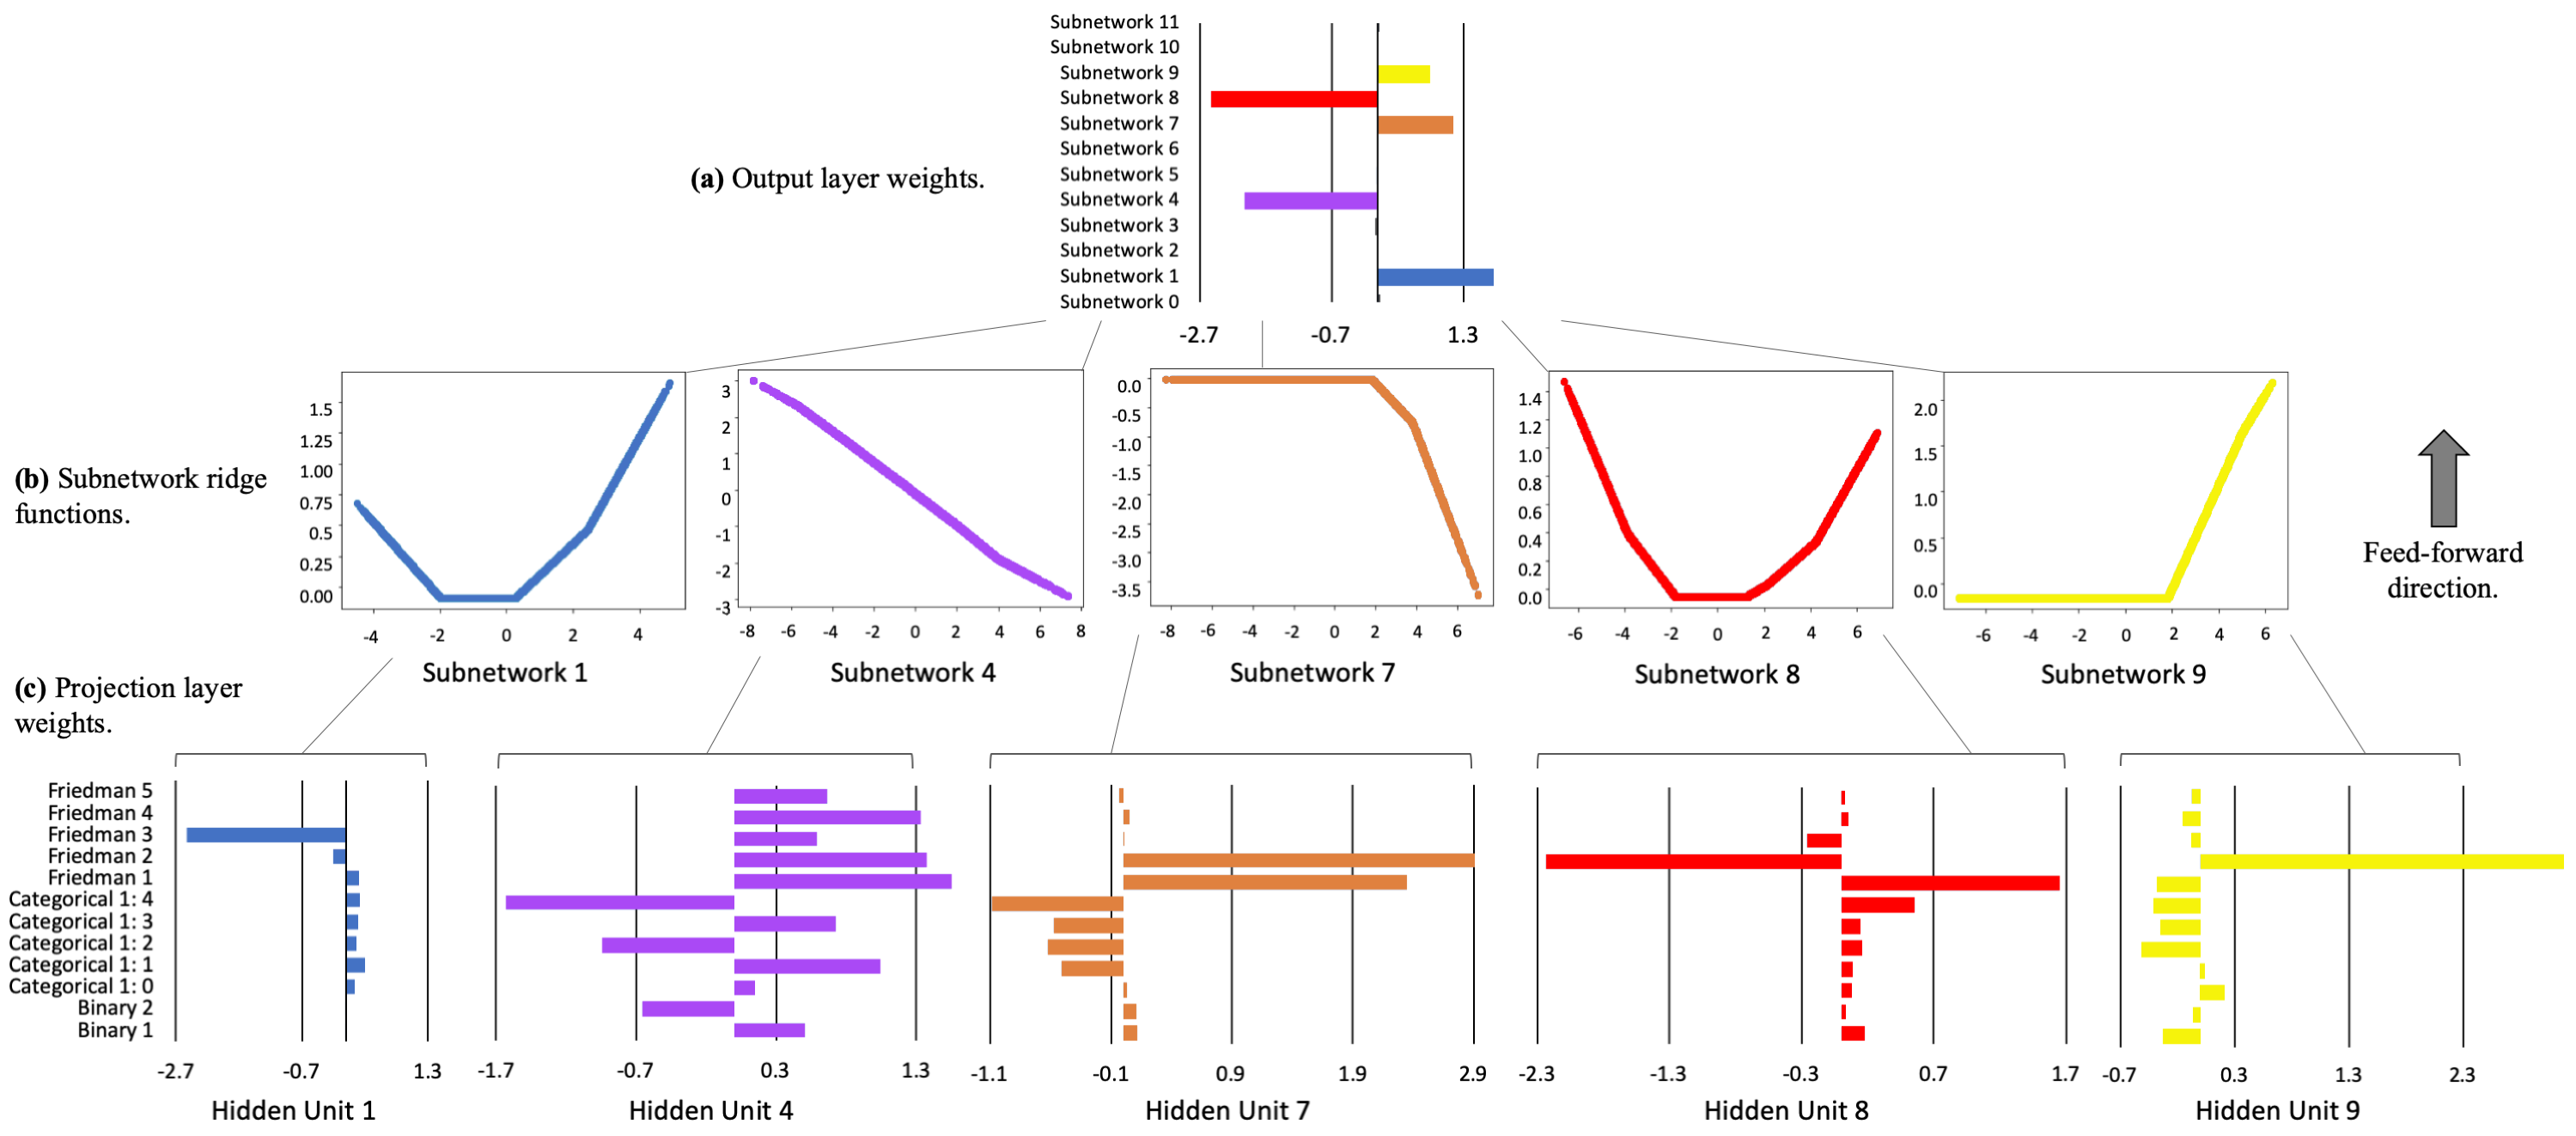
\includegraphics[width=18cm]{img/sim_xnn_glob_ridge.png}
	\caption{Output layer $\gamma_k$ weights, corresponding $n_k$ ridge functions, and associated projection layer $\beta_j$ weights for $g^\text{XNN}$ on the simulated test data.}
	\label{fig:sim_xnn_glob_ridge}
\end{figure} 

\noindent $n_k$ subnetworks are plotted across the output values of their associated $\sum_j\beta_{k,j}x_j$ projection layer hidden units, and color-coding between \ref{fig:sim_xnn_glob_ridge}\textbf{b} and \ref{fig:sim_xnn_glob_ridge}\textbf{c} link the $\beta_j$ weights to their $n_k$ subnetworks. Most of the heavily utilized $n_k$ subnetworks have sparse weights in their $\sum_j\beta_{k,j}x_j$ projection layer hidden units. In particular, subnetwork $n_1$ appears to be almost solely a function of $X_{\text{Friedman}, 3}$ and appears to exhibit the expected quadratic behavior for $X_{\text{Friedman}, 3}$.  Subnetworks $n_7$, $n_8$, and $n_9$ appear to be most associated with the globally important $X_{\text{Friedman}, 1}$ and $X_{\text{Friedman}, 2}$ features, likely betraying the effort required for $g^{\text{XNN}}$ to model the nonlinear $\text{sin}()$ function of the $X_{\text{Friedman}, 1}$ and $X_{\text{Friedman}, 2}$ product, and these subnetworks, especially $n_7$ and $n_8$, appear to display some noticeable sinusoidal characteristics. Subnetwork $n_4$ seems to be a linear combination of all the original input $X_j$ features, but does weigh the linear $X_{\text{Friedman},4}$ and $X_{\text{Friedman},5}$ terms roughly in the correct two-to-one ratio. As a whole, Figure \ref{fig:sim_xnn_glob_ridge}\textbf{a}, \textbf{b}, and \textbf{c} exhibit evidence that $g^\text{XNN}(\mathbf{X})$ has learned about the signal-generating function in Equation \ref{eq:sim} and the displayed information should help practitioners understand which original input $X_j$ features are weighed heavily in each $n_k$ subnetwork, and which $n_k$ subnetworks have a strong influence on $g^\text{XNN}(\mathbf{X})$ output. See Appendix \ref{a_ssec:xnn} for details regarding general XNN architecture.

%%%%%%%%%%%%%%%%%%%%%%%%%%%%%%%%%%%%%%%%%%
\subsection{Mortgage Data Results}

Results for the mortgage data are presented in Subsections \ref{ssec:c_v_uc_mort} -- \ref{ssec:dis_mort} to showcase the example workflow.  $g^\text{ANN}$ and $g^\text{XNN}$ outperform $g^\text{GBM}$ and $g^\text{MGBM}$ on the mortgage data, but as in Subsection \ref{ssec:c_v_uc_sim} the constrained variants of both model architectures do not show large differences in model fit with respect to unconstrained variants. Assuming that in high-stakes applications small fit differences on static test data do not outweigh the need for enhanced model debugging facilitated by high interpretability, only $g^\text{MGBM}$ and $g^\text{XNN}$ interpretability, post-hoc explainability, and discrimination testing results are presented. 

\subsubsection{Constrained vs. Unconstrained Model Fit Assessment}\label{ssec:c_v_uc_mort}

Table \ref{tab:mort_acc} shows that $g^\text{ANN}$ and $g^\text{XNN}$ noticeably outperform $g^\text{GBM}$ and $g^\text{MGBM}$ on the mortgage data for most of the fit measures. This is at least partially due to the preprocessing required to present directly comparable post-hoc explainability results and to use neural networks and tensorflow, e.g., numerical encoding of categorical features and missing values. This preprocessing appears to hamstring some of the tree-based models' inherent capabilities. $g^\text{GBM}$ models trained on non-encoded data with missing values repeatedly produced area under the curve (AUC) values of $\sim0.81$ (not shown, but available in resources discussed in Subsection \ref{ssec:soft}). 

\begin{table}[htb]
	\caption{Fit measures for $g^\text{GBM}$, $g^\text{MGBM}$, $g^\text{ANN}$, and $g^\text{XNN}$ on the mortgage test data. Arrows indicate the direction of improvement for each measure.}
\centering
\begin{tabular}{ccccccccc}
	\toprule
	\textbf{Model} & 
	\href{https://scikit-learn.org/stable/modules/model_evaluation.html#accuracy-score}{\textbf{Accuracy}}~$\uparrow$ & \href{https://en.wikipedia.org/wiki/Receiver_operating_characteristic#Area_under_the_curve}{\textbf{AUC}}~$\uparrow$ & \href{https://en.wikipedia.org/wiki/F1_score}{\textbf{F1}}~$\uparrow$ & 
	\href{https://scikit-learn.org/stable/modules/model_evaluation.html#log-loss}{\textbf{Logloss}}~$\downarrow$ & \href{https://en.wikipedia.org/wiki/Matthews_correlation_coefficient}{\textbf{MCC}}~$\uparrow$ & \href{https://en.wikipedia.org/wiki/Root-mean-square_deviation}{\textbf{RMSE}}~$\downarrow$ & \href{https://en.wikipedia.org/wiki/Sensitivity_and_specificity}{\textbf{Sensitivity}}~$\uparrow$ & \href{https://en.wikipedia.org/wiki/Sensitivity_and_specificity}{\textbf{Specificity}}~$\uparrow$ \\
	\midrule	
$g^\text{GBM}$		& 0.795	& 0.828	& 0.376 & 0.252 & 0.314 & 0.276 & 0.634 & 0.813 \\
$g^\text{MGBM}$	& 0.765	& 0.814	& 0.362 & 0.259 & 0.305 & 0.278 & 0.684 & 0.773 \\
$g^\text{ANN}$		& 0.865	& 0.871	& 0.474 & 0.231 & 0.418 & 0.262 & 0.624 & 0.891 \\
$g^\text{XNN}$		& 0.869	& 0.868	& 0.468 & 0.233 & 0.409 & 0.263 & 0.594 & 0.898 \\
\bottomrule
\label{tab:mort_acc}
\end{tabular}
\end{table}

\noindent Regardless of the fit differences between the two families of models, the difference between the constrained and unconstrained variants within the two types of models is small for the GBMs and smaller for the ANNs, $\sim$3.5\% and $\sim$1\% worse fit respectively, averaged across the measures in Table \ref{tab:mort_acc}.  

\subsubsection{Interpretability and Post-hoc Explanation Results}\label{ssec:int_ex_mort}

For $g^\text{MGBM}$, intrinsic interpretability is evaluated with PD and ICE plots of mostly monotonic prediction behavior for several important $X_j$, and post-hoc Shapley explanation analysis is used to create global and local feature importance. Global Shapley feature importance for $g^\text{MGBM}$ on the mortgage test data is reported in Figure \ref{fig:mort_mgbm_glob}. $g^\text{MGBM}$ places high importance on LTV ratio, perhaps too high, and also weighs DTI ratio, property value, loan amount, and introductory rate period heavily in many of its predictions. Tree SHAP values are reported in the margin space, prior to the application of the logit link function, and the reported numeric values can be interpreted as the mean absolute impact of each $X_j$ on $g^\text{MGBM}(\mathbf{X})$ in the mortgage test data in the $g^\text{MGBM}$ margin space. The potential over-emphasis of LTV ratio, and the de-emphasis of income, likely an important feature from a business perspective, and the encoded no introductory rate period flag feature may also contribute to the decreased performance of $g^\text{MGBM}$ as compared to $g^\text{XNN}$.

\begin{figure}[htb]
\centering
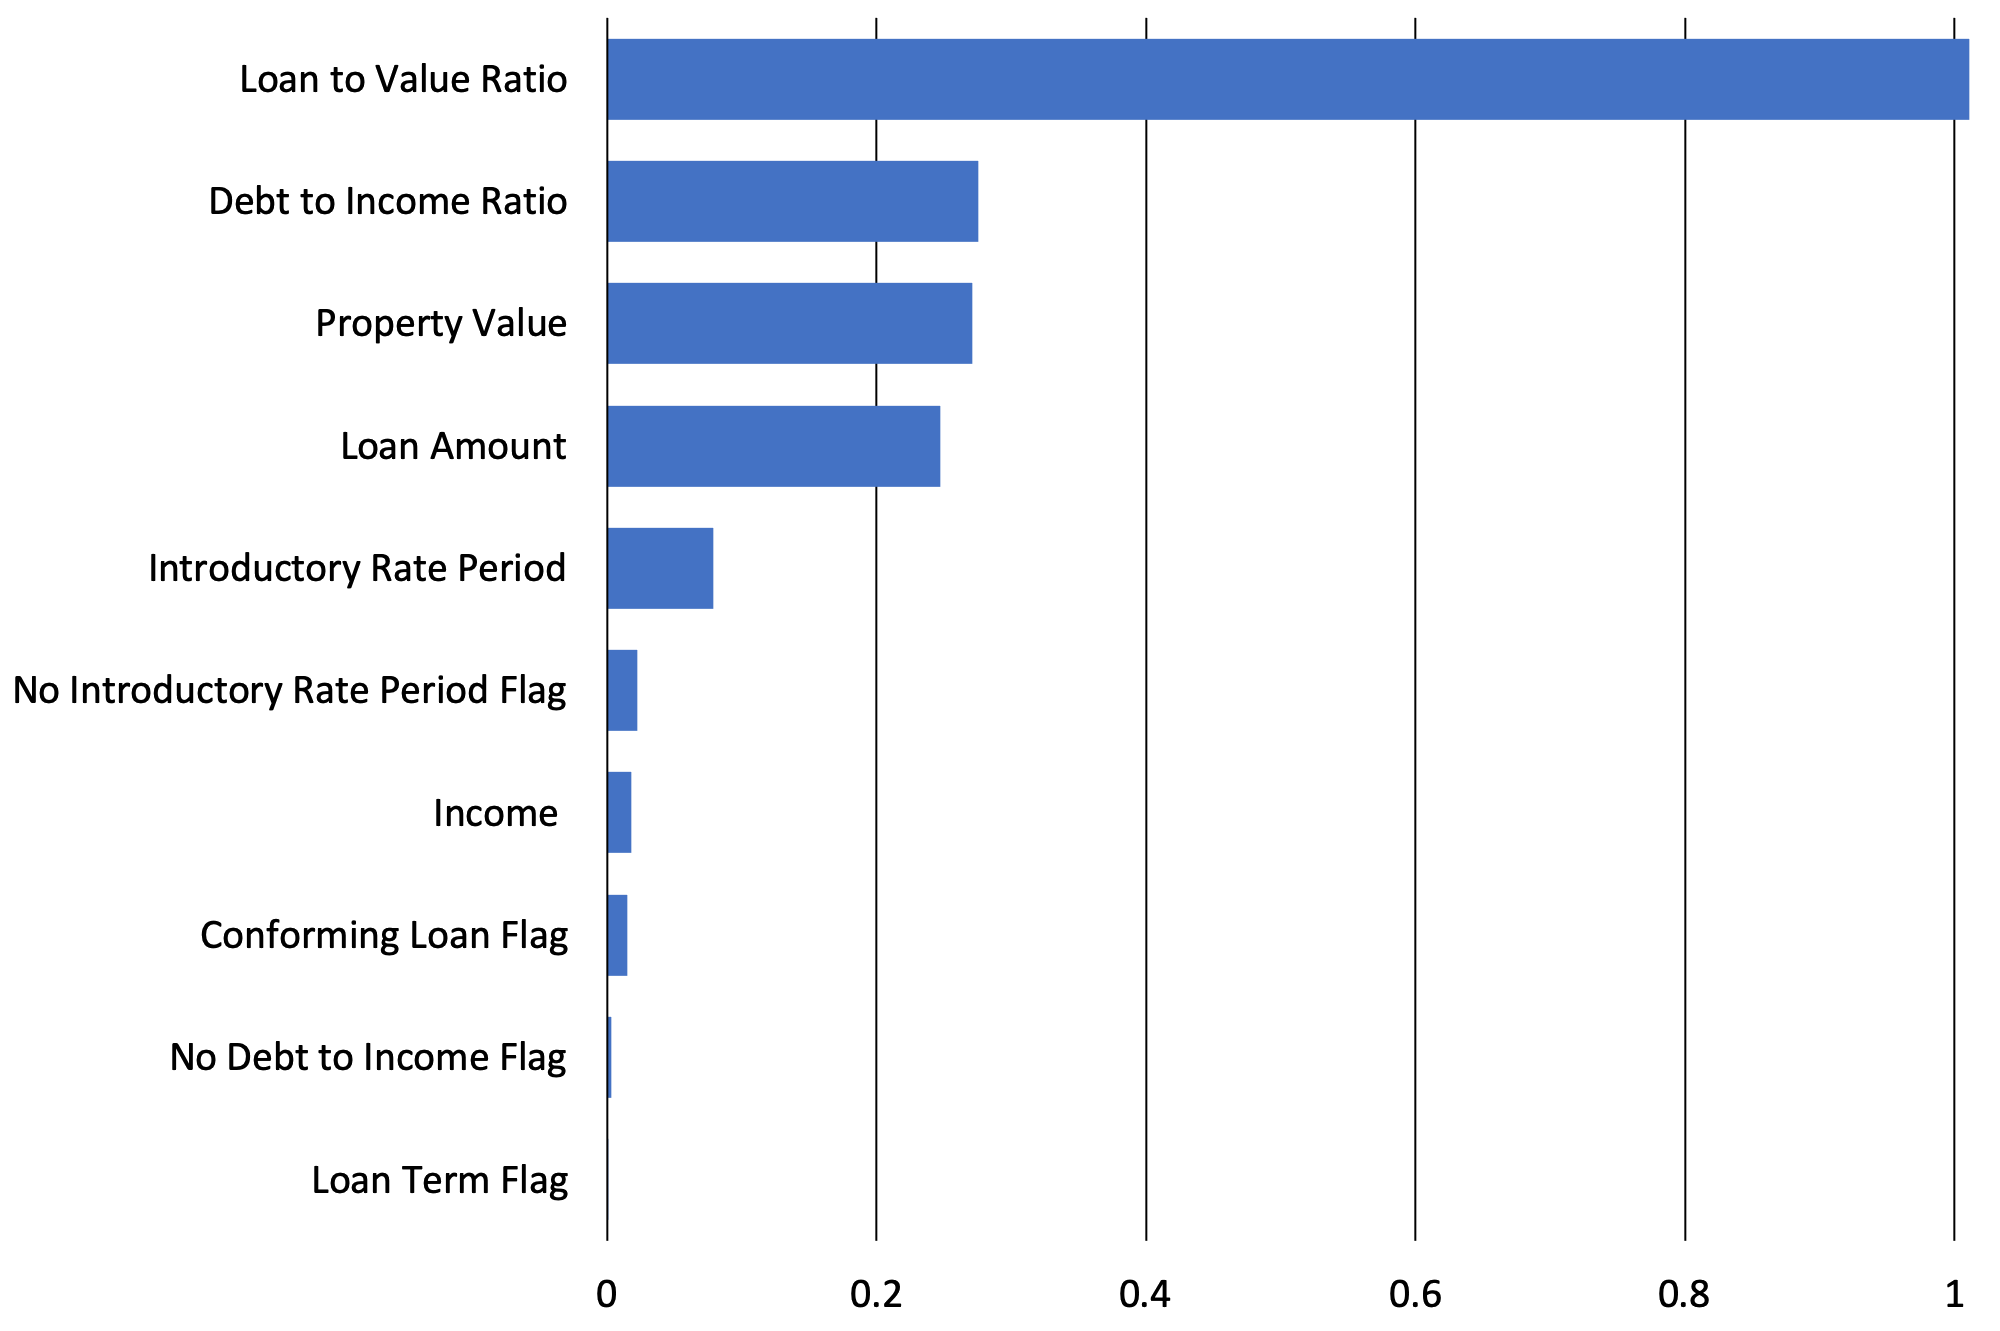
\includegraphics[width=9cm]{img/mort_mgbm_glob.png}
\caption{Global mean absolute Tree SHAP feature importance for $g^\text{MGBM}(\mathbf{X})$ on the mortgage test data.}
\label{fig:mort_mgbm_glob}
\end{figure} 

Domain knowledge was used to positively constrain DTI ratio and LTV ratio and to negatively constrain income and the loan term flag under $g^\text{MGBM}$. The monotonicity constraints for DTI ratio and LTV ratio are confirmed for $g^\text{MGBM}(\mathbf{X})$ on the mortgage test data in Figure \ref{fig:mort_mgbm_glob_pdp_ice}. Both DTI ratio and LTV ratio display positive monotonic behavior at all selected percentiles of $g^\text{MGBM}(\mathbf{X})$ for ICE and on average with PD. Because PD curves generally follow the patterns of the ICE curves for both features, it's also likely that no strong interactions are at play for DTI ratio and LTV ratio under $g^\text{MGBM}$. Of course, the monotonicity constraints themselves can dampen the effects of non-monotonic interactions under $g^\text{MGBM}$, even if they do exist in the data. Perhaps due to the presence of important non-monotonic interactions (e.g., LTV ratio and the no introductory rate period flag, see Figure \ref{fig:mort_xnn_glob_ridge}). This rigidity could also play a role in the performance differences between $g^\text{MGBM}$ and $g^\text{XNN}$ in the mortgage data not observed for the simulated data, wherein strong interactions appear to be between features with the same monotonicity constraints (e.g., $X_{\text{Friedman},1}$ and $X_{\text{Friedman},2}$, see Figure \ref{fig:sim_xnn_glob_ridge}).

PD and ICE are displayed with a histogram to highlight any sparse regions in an input feature's domain. Because most ML models will always issue a prediction on any instance with a correct schema, it's crucial to consider whether a given model learned enough about an observation to make an accurate prediction. Viewing PD and ICE along with a histogram is a convenient method to visually assess whether a prediction is reasonable and based on sufficient training data. DTI ratio and LTV ratio do appear to have sparse regions in their univariate distributions. The monotonicity constraints likely play to the advantage of $g^\text{MGBM}$ in this regard, as $g^\text{MGBM}$ appears to carry reasonable predictions learned from populous domains into the sparse domains of both features. 

\begin{figure}[htb]
\hskip-10pt\includegraphics[width=16.5cm]{img/mort_mgbm_glob_pdp_ice.png}
\caption{PD, ICE for 10 individuals across selected percentiles of $g^\text{MGBM}(\mathbf{X})$, and histograms for the three most important input features of $g^\text{MGBM}$ on the mortgage test data.}
\label{fig:mort_mgbm_glob_pdp_ice}
\end{figure}   

Figure \ref{fig:mort_mgbm_glob_pdp_ice} also displays PD and ICE for the unconstrained feature property value. Unlike DTI ratio and LTV ratio, PD for property value does not always follow the patterns established by ICE curves. While PD shows monotonically increasing prediction behavior on average, apparently influenced by large predictions at extreme $g^{\text{MGBM}}(\mathbf{X})$ percentiles, ICE curves for individuals at the 40\textsuperscript{th} percentile of $g^{\text{MGBM}}(\mathbf{X})$, and lower, exhibit different prediction behavior with respect to property value. Some individuals at these lower percentiles display monotonically decreasing prediction behavior while others appear to show fluctuating prediction behavior. Property value is strongly right-skewed, with little data regarding high-value property from which $g^{\text{MGBM}}$ can learn. For the most part, reasonable predictions do appear to be carried from more densely populated regions to more sparsely populated regions. However, prediction fluctuations at lower $g^{\text{MGBM}}(\mathbf{X})$ percentiles are visible, and appear in a sparse region of property value. This divergence of PD and ICE can be indicative of an interaction affecting property value under $g^{\text{MGBM}}$ \cite{ice_plots}, and analysis by surrogate decision tree did show evidence of numerous potential interactions in lower predictions ranges of $g^{\text{MGBM}}(\mathbf{X})$ \cite{art_and_sci} (not shown, but available in resources discussed in Subsection \ref{ssec:soft}). However, fluctuations in ICE can also be caused by overfitting or by leakage of strong non-monotonic signal from important constrained features into the modeled behavior of non-constrained features. 

In Figure \ref{fig:mort_mgbm_loc}, local Tree SHAP values are displayed for selected individuals at the 10\textsuperscript{th}, 50\textsuperscript{th}, and 90\textsuperscript{th} percentiles of $g^{\text{MGBM}}(\mathbf{X})$ in the mortgage test data. Each $\phi_j$ value in Figure \ref{fig:mort_mgbm_loc} represents the difference in $g^\text{MGBM}(\mathbf{x^{(i)}})$ and the average of $g^\text{MGBM}(\mathbf{X})$ associated with some input feature $X_j$ \cite{molnar}. Accordingly, the logit of the sum of the Shapley values and the Shapley intercept will be the $g^\text{MGBM}(\mathbf{x})$ prediction in the probability space, for any $\mathbf{x}$. 

\begin{figure}[htb]
\centering
\includegraphics[width=16cm]{img/mort_mgbm_loc.png}
\caption{Tree SHAP values for three individuals across selected percentiles of $g^\text{MGBM}(\mathbf{X})$ for the mortgage test data.}
\label{fig:mort_mgbm_loc}
\end{figure}   

\noindent The selected individuals show an expected progression of mostly negative Shapley values at the 10\textsuperscript{th} percentile, a mixture of positive and negative Shapley values at the 50\textsuperscript{th} percentile, mostly positive Shapley values the 90\textsuperscript{th} percentile, and with globally important features driving most local model decisions. Deeper significance for Figure \ref{fig:mort_mgbm_loc} lies in the ability of Tree SHAP to accurately and consistently summarize any single $g^\text{MGBM}(\mathbf{x})$ prediction in this manner, which is generally important for enabling logical appeal or override of ML-based decisions, and is specifically important in the context of lending, where applicable regulations often require lenders to provide consumer-specific reasons for denying credit to an individual. In the US, applicable regulations are typically ECOA and FCRA, and the consumer-specific reasons are commonly known as adverse actions codes.

Figure \ref{fig:mort_xnn_glob} displays global feature importance for $g^\text{XNN}$ on the mortgage test data. Deep SHAP values are reported in the probability space, after the application of the logit link function. They are also calculated from the projection layer of $g^\text{XNN}$. Thus, the Deep SHAP values in Figure \ref{fig:mort_xnn_glob} are the estimated average absolute impact of each $X_j$ in the projection layer and probability space of $g^\text{XNN}$ for the mortgage test data. $g^\text{XNN}$ distributes importance more evenly across business drivers and puts stronger emphasis on the no introductory rate period flag feature than does $g^\text{MGBM}$. Like $g^\text{MGBM}$, $g^\text{XNN}$ puts little emphasis on the other flag features.  

\begin{figure}[htb]
\centering
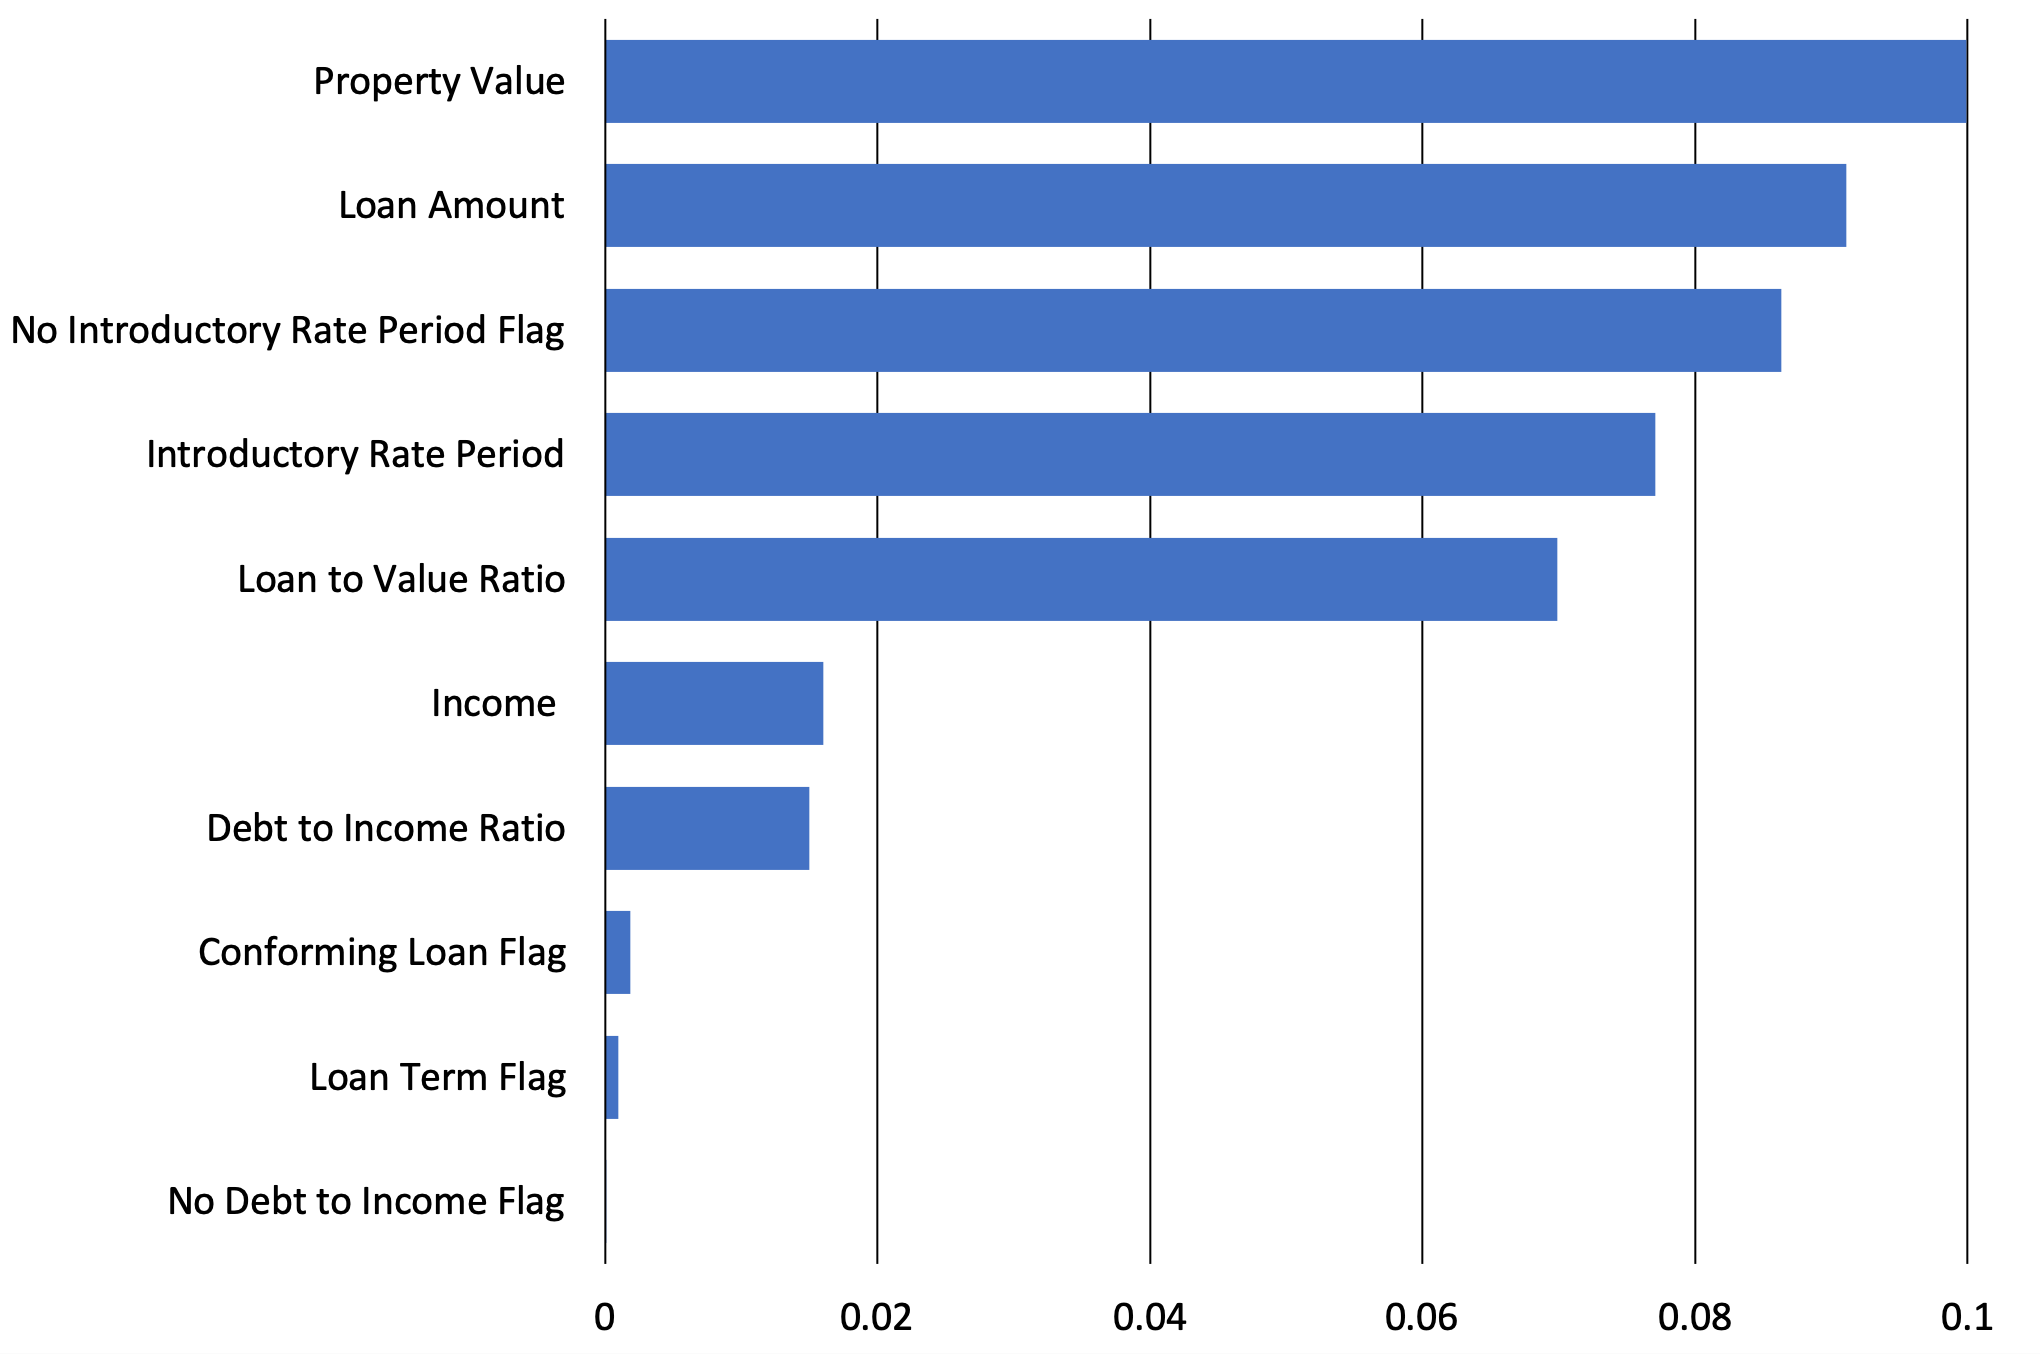
\includegraphics[width=9cm]{img/mort_xnn_glob.png}
\caption{Global mean absolute Deep SHAP feature importance for $g^\text{XNN}(\mathbf{X})$ on the mortgage test data.}
\label{fig:mort_xnn_glob}
\end{figure} 

\noindent As compared to $g^\text{MGBM}$, $g^\text{XNN}$ assigns higher importance to property value, loan amount, and income, and lower importance on LTV ratio and DTI ratio. 

The capability of $g^\text{XNN}$ to model nonlinear phenomenon and high-degree interactions, and to do so in an interpretable manner, is on display in Figure \ref{fig:mort_xnn_glob_ridge}. \ref{fig:mort_xnn_glob_ridge}\textbf{a} presents the sparse $\gamma_k$ weights of the $g^\text{XNN}$ output layer in which the $n_k$ subnetworks with $k \in \{0,1,2,3,5,8,9\}$ have large magnitude weights and $n_k$ subnetworks, $k \in \{4,6,7\}$, have small or near-zero magnitude weights. Distinctive ridge functions that feed into those large magnitude $\gamma_k$ weights are highlighted in \ref{fig:mort_xnn_glob_ridge}\textbf{b} and color-coded to pair with their corresponding $\gamma_k$ weight. As in the Subsection \ref{ssec:xnn_sim}, $n_k$ ridge function plots vary with the output of the corresponding projection layer $\sum_j\beta_{k,j}x_j$ hidden unit, with weights displayed in matching colors in \ref{fig:mort_xnn_glob_ridge}\textbf{c}. In both the simulated and mortgage data, $n_k$ ridge functions appear to be elementary functional forms that the output layer learns to combine to generate accurate predictions, reminiscent of basis functions for the modeled space. \ref{fig:mort_xnn_glob_ridge}\textbf{c} displays the sparse $\beta_j$ weights of the projection layer $\sum_j\beta_{k,j}x_j$ hidden units that are associated with each $n_k$ subnetwork ridge function. For instance, subnetwork $n_3$ is influenced by large weights for LTV ratio, no introductory rate period flag, and introductory rate period, whereas subnetwork $n_9$ is nearly completely dominated by the weight for income. See Appendix \ref{a_ssec:xnn} for details regarding general XNN architecture.

\begin{figure}[htb]
\hskip-20pt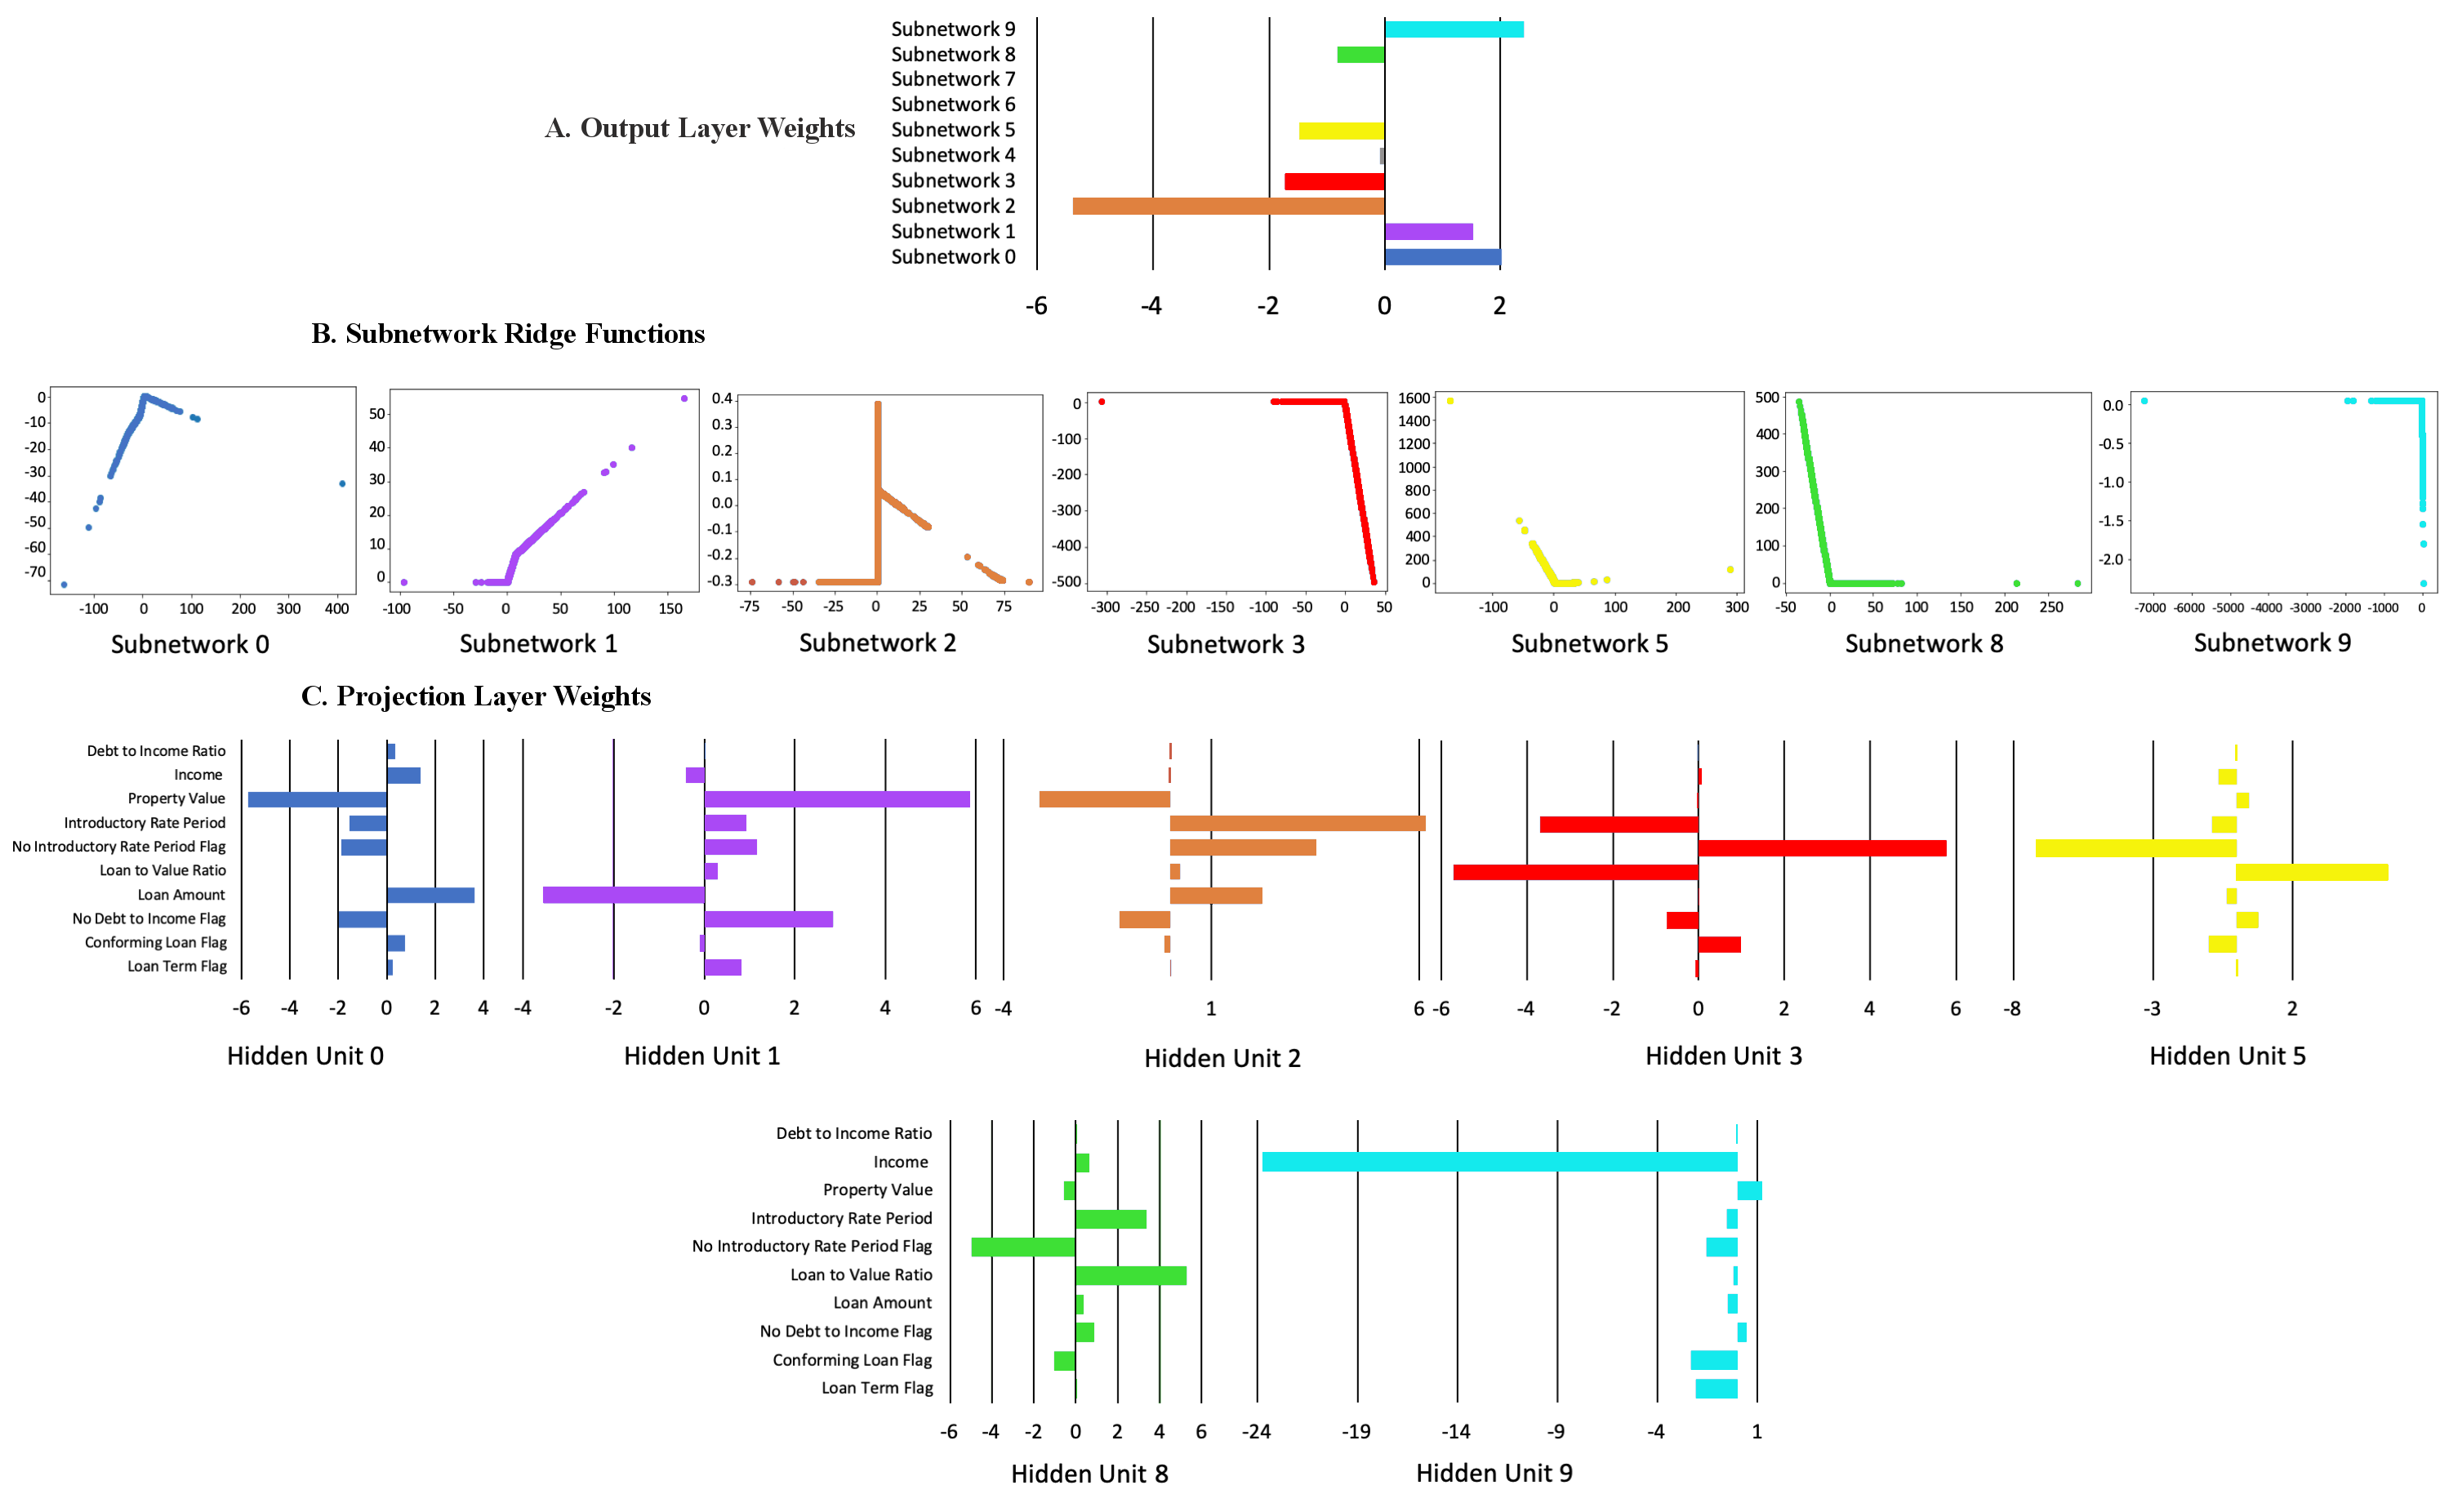
\includegraphics[width=18cm]{img/mort_xnn_glob_ridge.png}
\caption{Output layer $\gamma_k$ weights, corresponding $n_k$ ridge functions, and associated projection layer $\beta_j$ weights for $g^\text{XNN}$ on the mortgage test data.}
\label{fig:mort_xnn_glob_ridge}
\end{figure} 

To compliment the global interpretability of $g^\text{XNN}$, Figure \ref{fig:mort_xnn_loc} displays local Shapley values for selected individuals, estimated from the projection layer using Deep SHAP in the $g^\text{XNN}$ probability space. Similar to Tree SHAP, local Deep SHAP values should sum to $g^\text{XNN}(\mathbf{x})$. While the Shapley values appear to follow the roughly increasing pattern established in Figures \ref{fig:sim_mgbm_loc}, \ref{fig:sim_xnn_loc}, and \ref{fig:mort_mgbm_loc}, their true value is their ability to be calculated for any $g^\text{XNN}(\mathbf{x})$ prediction, as a means to summarize model reasoning and allow for appeal and override of specific ML-based decisions, even for neural network architectures. 

\begin{figure}[htb]
\centering
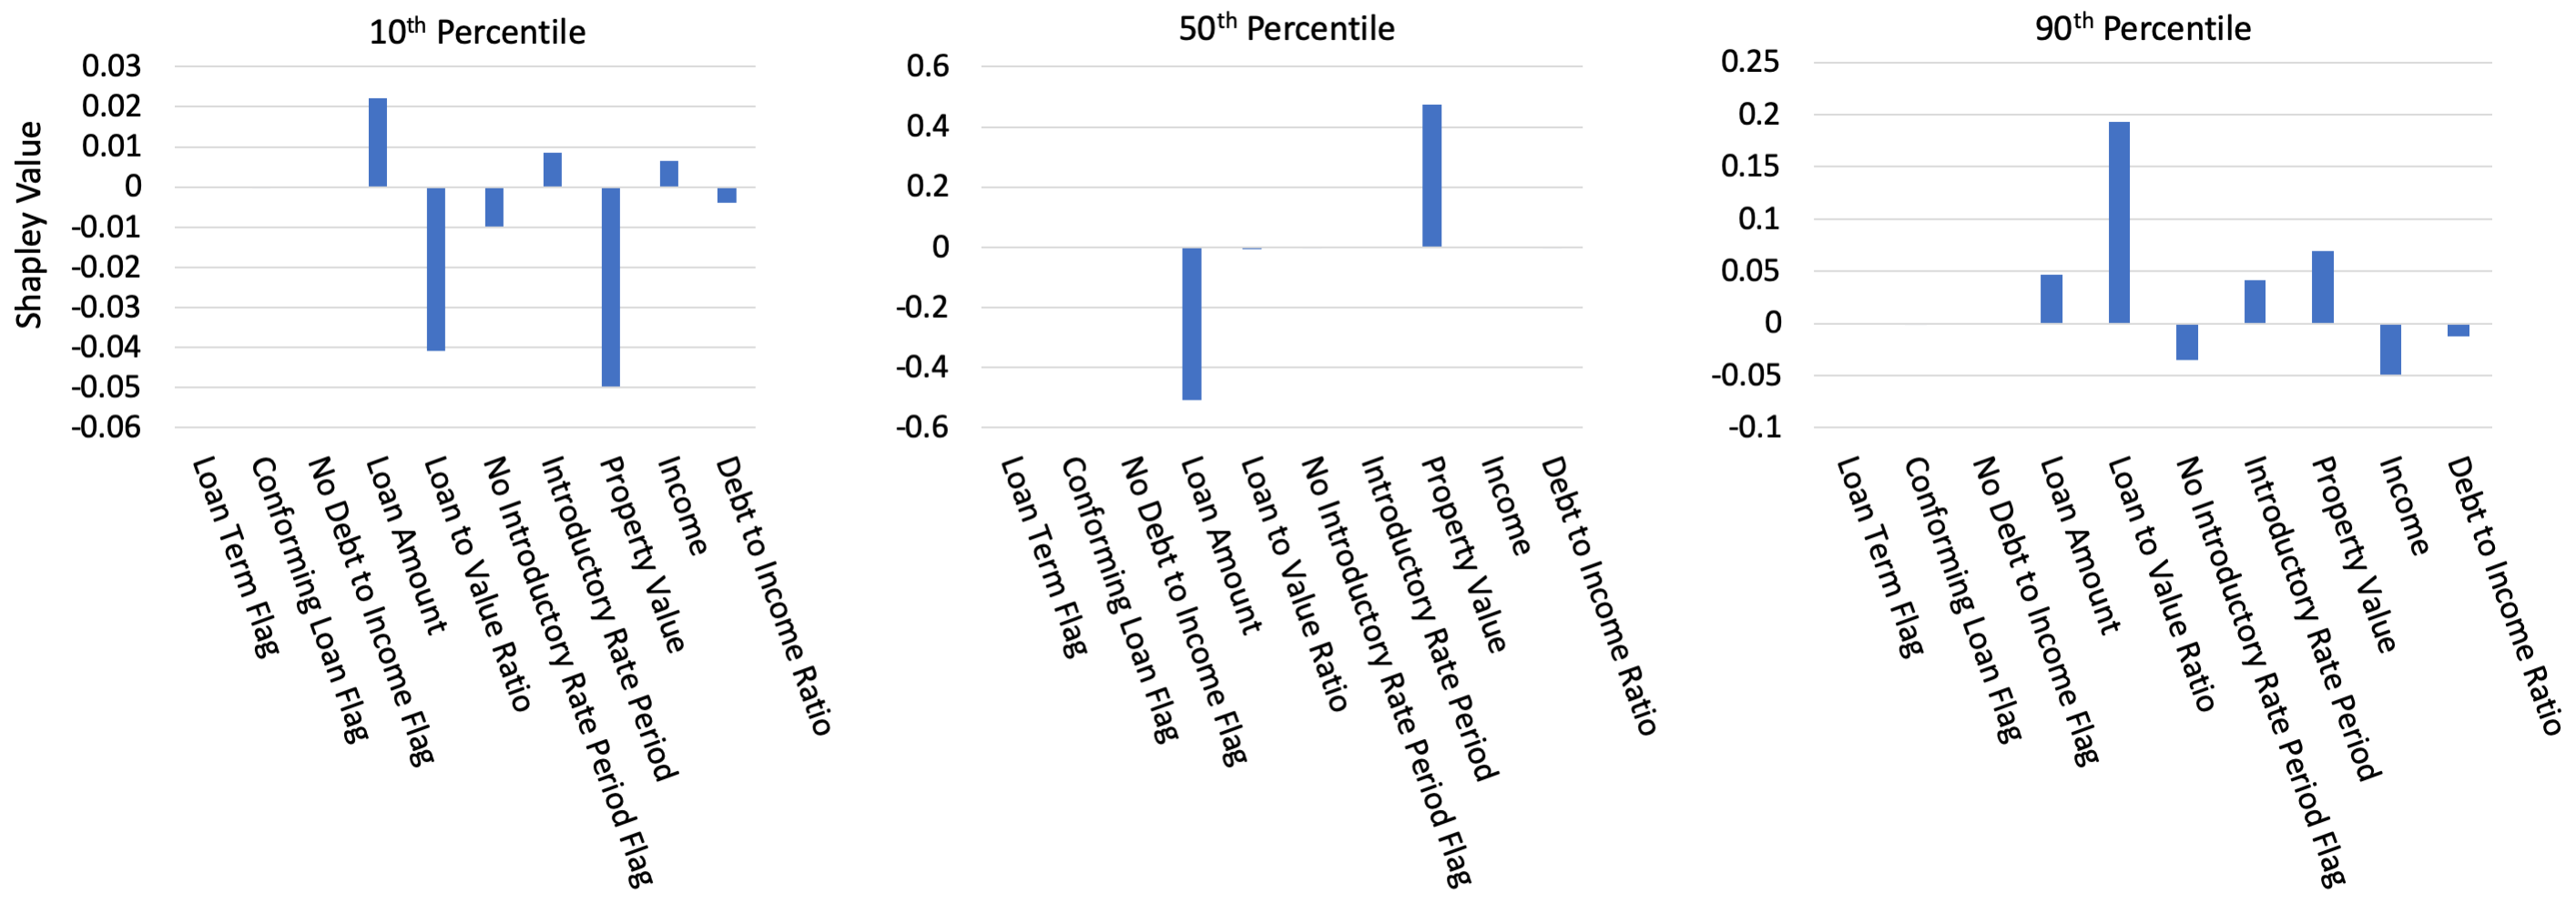
\includegraphics[width=16cm]{img/mort_xnn_loc.png}
\caption{Deep SHAP values for three individuals across selected percentiles of $g^\text{XNN}(\mathbf{X})$ on the mortgage test data.}
\label{fig:mort_xnn_loc}
\end{figure}

\subsubsection{Discrimination Testing Results}\label{ssec:dis_mort}

Tables \ref{tab:mort_disc}\textbf{a} and \ref{tab:mort_disc}\textbf{b} show the results of the discrimination tests using the mortgage data for two sets of class-control groups: blacks as compared to whites, and females as compared to males. As with the simulated data in Table \ref{tab:sim_disc}, several measures of disparities are shown, with the SMDs calculated using the probabilities from $g^{\text{MGBM}}$ and $g^{\text{XNN}}$, and the accuracy, FPRs, and  FPR ratios, MEs, and AIRs calculated using a binary outcome based on a cutoff of 0.20 (anyone with probabilities of 0.2 or less receives the favorable outcome).\footnote{See Appendix \ref{a_sec:cut} for comments pertaining to discrimination testing and cutoff selection.} Since $g^{\text{MGBM}}$ and $g^{\text{XNN}}$  are predicting the likelihood of receiving a high-priced loan, $g^{\text{MGBM}}$ and $g^{\text{XNN}}$ assume that a lower score is favorable.  Thus, one might consider FPR ratios as a measure of the class-control disparities. FPR ratios are higher under $g^{\text{XNN}}$ than $g^{\text{MGBM}}$ (2.45 vs. 2.10) in Table \ref{tab:mort_disc}\textbf{b}, but overall FPRs are lower for blacks under $g^{\text{XNN}}$ (0.295 vs. 0.315) in Table \ref{tab:mort_disc}\textbf{a}.  This is the same pattern seen in the simulated data results in Appendix \ref{a_ssec:dis_sim}, again leading to the question of whether a fairness goal should not only consider class-control relative rates, but also intra-class improvements in the chosen fairness metric.  Similar results are found for the female-male comparison, but the relative rates are less stark: 1.15 for $g^{\text{MGBM}}$ and 1.21 for $g^{\text{XNN}}$.

\begin{table}[htb]
	\hskip-10pt\begin{subtable}{0.45\textwidth}
	\captionsetup{width=7cm}
	\caption{Group size, accuracy, and FPR for $g^\text{MGBM}$ and $g^\text{XNN}$ on the mortgage test data.} 
	\centering
	\resizebox{\columnwidth}{!}{%
	\begin{tabular}{ccccc}
		\toprule
		\textbf{Class} & $\mathbf{N}$ & \textbf{Model} & \textbf{Accuracy}$\uparrow$ & \textbf{FPR}$\downarrow$ \\
		\midrule
		Black & 2,608 & \begin{tabular}{@{}c@{}} $g^\text{MGBM}$ \\ $g^\text{XNN}$\end{tabular}	& \begin{tabular}{@{}c@{}} 0.654 \\ 0.702\end{tabular} & \begin{tabular}{@{}c@{}} 0.315 \\ 0.295\end{tabular} \\	
		\midrule			 
		White & 28,361 & \begin{tabular}{@{}c@{}} $g^\text{MGBM}$ \\ $g^\text{XNN}$\end{tabular} & \begin{tabular}{@{}c@{}} 0.817 \\ 0.857\end{tabular} & \begin{tabular}{@{}c@{}} 0.150 \\ 0.120\end{tabular}\\		
		\midrule
		Female & 8,301 & \begin{tabular}{@{}c@{}} $g^\text{MGBM}$ \\ $g^\text{XNN}$\end{tabular} & \begin{tabular}{@{}c@{}}  0.768 \\ 0.822\end{tabular} & \begin{tabular}{@{}c@{}} 0.208 \\ 0.158\end{tabular}\\
		\midrule
		Male & 13,166 & \begin{tabular}{@{}c@{}} $g^\text{MGBM}$ \\ $g^\text{XNN}$\end{tabular}	& \begin{tabular}{@{}c@{}} 0.785 \\ 0.847\end{tabular} & \begin{tabular}{@{}c@{}} 0.182 \\ 0.131\end{tabular}\\
		\bottomrule
		\label{tab:mort_n_acc}
	\end{tabular}%
	}
	\end{subtable}
	\hspace{10pt}
	\begin{subtable}{0.45\textwidth}
	\vspace{-14pt}
	\captionsetup{width=10cm}
	\caption{%
		\leftskip=45pt
		AIR, ME, SMD, and FPR ratio for $g^\text{MGBM}$ and $g^\text{XNN}$ on the mortgage test data.}
	\centering
	\scalebox{0.95}{
	\begin{tabular}{ccccccc}
		\toprule
		\textbf{Model} &  \begin{tabular}[x]{@{}c@{}}\textbf{Protected}\\\textbf{Class}\end{tabular} & \begin{tabular}[x]{@{}c@{}}\textbf{Control}\\\textbf{Class}\end{tabular} & \textbf{AIR}$\uparrow$ & \textbf{ME}$\downarrow$ & \textbf{SMD}$\downarrow$ & \begin{tabular}[x]{@{}c@{}}\textbf{FPR}\\\textbf{Ratio}\end{tabular}$\downarrow$\\
		\midrule
		$g^\text{MGBM}$	& \begin{tabular}{@{}c@{}} Black \\ Female\end{tabular}	& \begin{tabular}{@{}c@{}} White \\ Male\end{tabular} & \begin{tabular}{@{}c@{}} 0.776 \\ 0.948\end{tabular} & \begin{tabular}{@{}c@{}} 18.3\% \\ 4.1\%\end{tabular}	& \begin{tabular}{@{}c@{}} 0.628 \\ 0.084\end{tabular} & \begin{tabular}{@{}c@{}} 2.10 \\ 1.15\end{tabular} \\
		\midrule 
		$g^\text{XNN}$ & \begin{tabular}{@{}c@{}} Black \\ Female\end{tabular} & \begin{tabular}{@{}c@{}} White \\ Male\end{tabular} & \begin{tabular}{@{}c@{}} 0.743 \\ 0.955\end{tabular} & \begin{tabular}{@{}c@{}} 21.4\% \\ 3.6\%\end{tabular} & \begin{tabular}{@{}c@{}} 0.621 \\ 0.105\end{tabular} & \begin{tabular}{@{}c@{}} 2.45 \\ 1.21\end{tabular} \\							
		\bottomrule
		\label{tab:mort_disc_detail}
	\end{tabular}
	}
	\end{subtable}
\captionsetup{width=10cm}
\caption{Discrimination measures for the mortgage test data. Arrows indicate the direction of improvement for each measure.}
\label{tab:mort_disc}
\end{table}

Both ME and AIR show higher disparities for blacks under $g^{\text{XNN}}$ than $g^{\text{MGBM}}$.  Blacks receive high-priced loans 21.4\% more frequently using $g^{\text{XNN}}$ vs. 18.3\% for $g^{\text{MGBM}}$.  Both $g^{\text{MGBM}}$ and $g^{\text{XNN}}$ show AIRs that are statistically significantly below parity (not shown, but available in resources discussed in Subsection \ref{ssec:soft}), and which are also below the EEOC’s 0.80 threshold. This would typically indicate need for further review to determine the cause and validity of these disparities, and a few relevant remediation techniques for such discovered discrimination are discussed in Subsection \ref{ssec:disc_rem}. On the other hand, women improve under $g^{\text{XNN}}$ vs. $g^{\text{MGBM}}$ (MEs of 3.6\% vs. 4.1\%; AIRs of 0.955 vs. 0.948). The AIRs, while statistically significantly below parity, are well above the EEOC’s threshold of 0.80.  In most situations, the values of these metrics alone would not likely flag a model for further review. Black SMDs for $g^{\text{XNN}}$ and $g^{\text{MGBM}}$ are similar: 0.621 and 0.628, respectively.  These exceed Cohen’s guidelines of 0.5 for a medium effect size and would likely trigger further review.  Female SMDs are well below Cohen’s definition of small effect size: 0.105 and 0.084 for $g^{\text{XNN}}$ and $g^{\text{MGBM}}$, respectively.  Similar to results for female AIR, these values alone are unlikely to prompt further review.

%%%%%%%%%%%%%%%%%%%%%%%%%%%%%%%%%%%%%%%%%%
\section{Discussion}\label{sec:disc}

\subsection{The Burgeoning Python Ecosystem for Responsible Machine Learning}

Figure \ref{fig:blueprint} displays a holistic approach to ML model training, assessment, deployment meant to decrease discrimination, inaccuracy, privacy, and security risks for high-stakes, human-centered, or regulated ML applications.\footnote{See: \href{https://github.com/jphall663/hc_ml}{Toward Responsible Machine Learning} for details regarding Figure \ref{fig:blueprint}.} While all the methods mentioned in Figure \ref{fig:blueprint} play an important role in increasing human trust and understanding of ML, a few pertinent references and Python resources are highlighted below as further reading to augment this this text's focus on certain interpretable models, post-hoc explanation, and discrimination testing techniques.   

\begin{figure}[H]
	\centering
	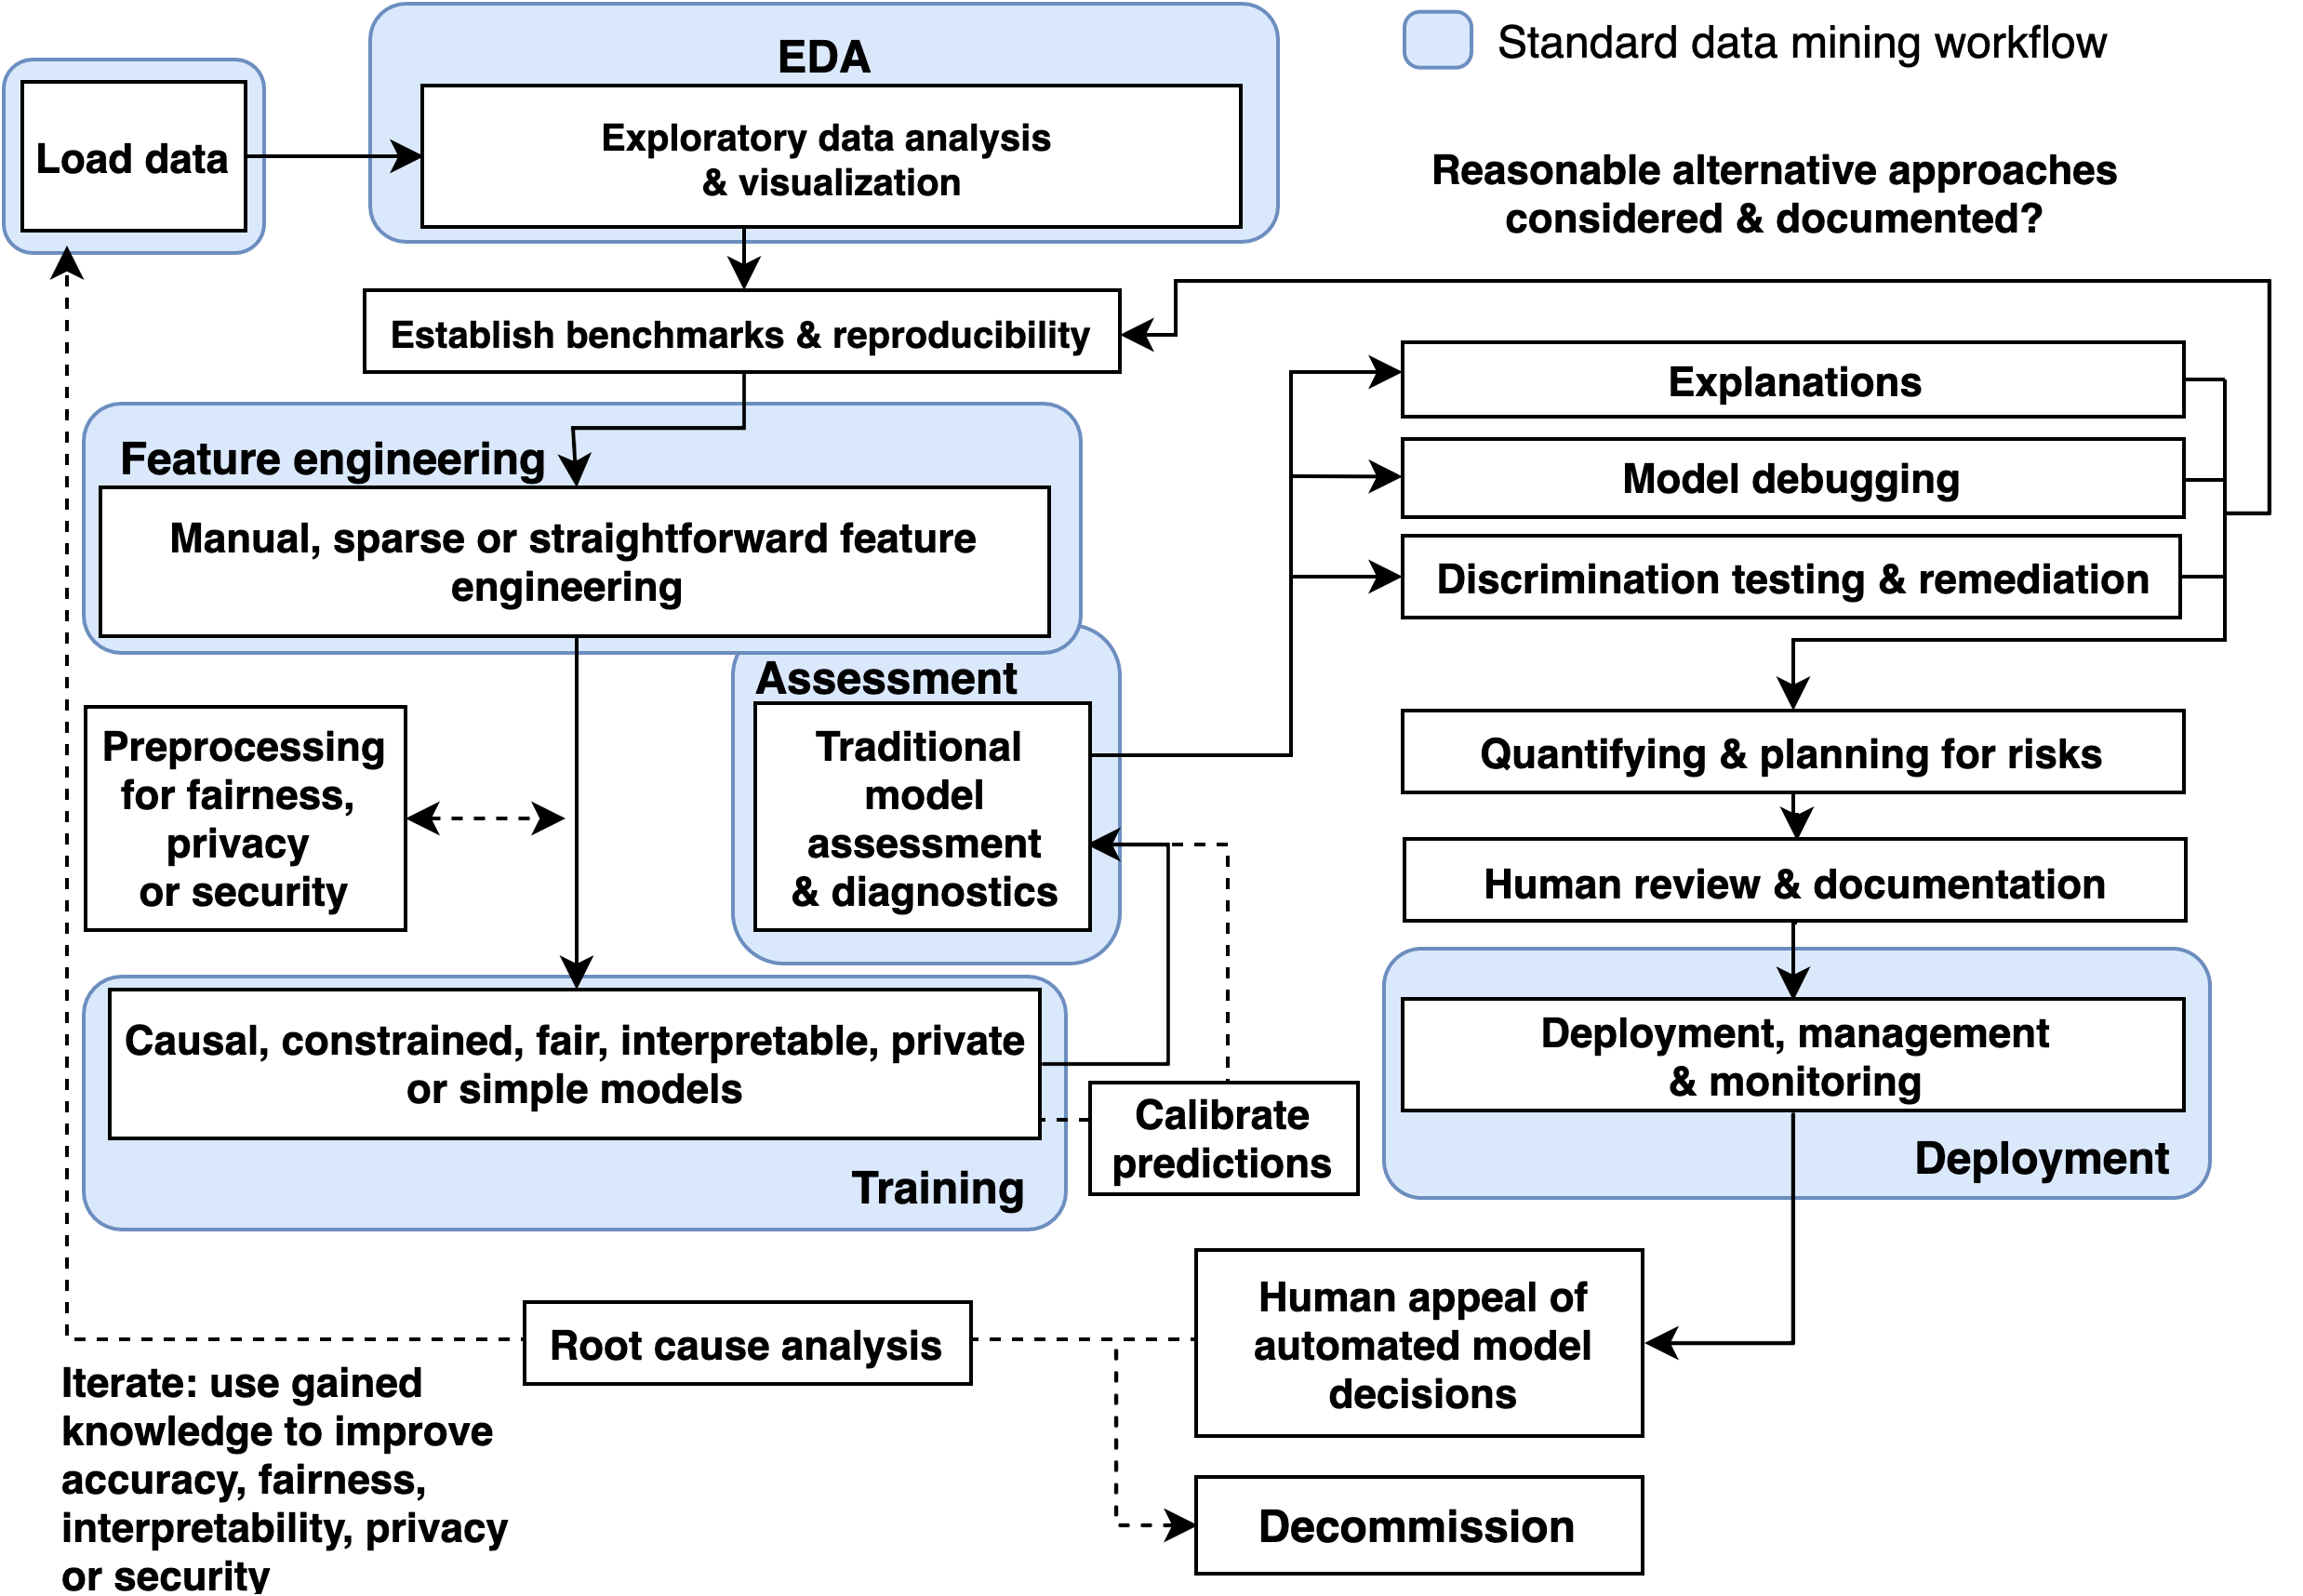
\includegraphics[width=11cm]{img/blueprint.png}
	\caption{An example responsible ML workflow in which interpretable models, post-hoc explanations, discrimination testing and remediation techniques, among other review and appeal mechanisms, can create an understandable and trustworthy ML system.}
	\label{fig:blueprint}
\end{figure} 

Any discussion of interpretable ML models would be incomplete without references to the seminal work of the Rudin group at Duke University and EBM, or GA\textsuperscript{2}M models, pioneered by researchers at Microsoft and Cornell. In keeping with a major theme of this manuscript, models from these leading researchers and several other kinds of interpretable ML models are now available as open source Python packages. Among several types of currently available interpretable models, practitioners can now use Python to evaluate EBM in the \href{https://github.com/interpretml/interpret}{\texttt{interpret}} package, optimal sparse decision trees, GAMs in the \href{https://github.com/dswah/pyGAM}{\texttt{pyGAM}} package, a variant of Friedman's RuleFit  in the \href{https://github.com/scikit-learn-contrib/skope-rules}{\texttt{skope-rules}} package, monotonic calibrated interpolated lookup tables in \href{https://github.com/tensorflow/lattice}{\texttt{tensorflow/lattice}}, and \textit{this looks like that} interpretable deep learning \cite{osdt}, \cite{rulefit}, \cite{lattice}, \cite{this_looks_like_that}.\footnote{See: \href{https://github.com/xiyanghu/OSDT}{Optimal sparse decision trees}.}\textsuperscript{,}\footnote{See: \href{https://github.com/cfchen-duke/ProtoPNet}{\textit{This looks like that} interpretable deep learning}.} Additional, relevant references and Python functionality include:

\begin{itemize}[leftmargin=*,labelsep=5.8mm]

\item \textbf{Exploratory data analysis (EDA)}: \texttt{H2OAggregatorEstimator} in \href{http://docs.h2o.ai/h2o/latest-stable/h2o-py/docs/modeling.html#h2oaggregatorestimator}{\texttt{h2o}} \cite{wilkinson2018visualizing}.

\item \textbf{Sparse feature extraction}: \texttt{H2OGeneralizedLowRankEstimator} in \href{http://docs.h2o.ai/h2o/latest-stable/h2o-py/docs/modeling.html#h2ogeneralizedlowrankestimator}{\texttt{h2o}} \cite{udell2016generalized}.

\item \textbf{Privacy preprocessing and private models}: differential privacy and private models in \href{https://github.com/IBM/differential-privacy-library}{\texttt{diffprivlib}} and \href{https://github.com/tensorflow/privacy/}{\texttt{tensorflow/privacy}} \cite{diffprivlib}, \cite{ji2014differential}, \cite{pate}, \cite{abadi2016deep}.

\item \textbf{Post-hoc explanation}: structured data explanations with \href{https://github.com/SeldonIO/alibi}{\texttt{alibi}} and \href{https://github.com/SauceCat/PDPbox}{\texttt{PDPbox}}, image classification explanations with \href{https://github.com/marcoancona/DeepExplain}{\texttt{DeepExplain}}, and natural language explanations with \href{https://github.com/allenai/allennlp}{\texttt{allennlp}} \cite{wachter2017counterfactual}, \cite{grad_attr}, \cite{wallace2019allennlp}. 

\item \textbf{Discrimination testing}: with \href{https://github.com/dssg/aequitas}{\texttt{aequitas}} and \href{https://github.com/LASER-UMASS/Themis}{\texttt{Themis}}.

\item \textbf{Discrimination remediation}: Reweighing, adversarial de-biasing, learning fair representations, and reject option classification with \href{http://aif360.mybluemix.net/}{\texttt{AIF360}} \cite{kamiran2012data}, \cite{zhang2018mitigating}, \cite{lfr}, \cite{kamiran2012decision}.

\item \textbf{Model debugging}: with \href{https://github.com/bethgelab/foolbox}{\texttt{foolbox}}, \href{https://github.com/SALib/SALib}{\texttt{SALib}}, \href{https://github.com/tensorflow/cleverhans}{\texttt{tensorflow/cleverhans}}, and \href{https://github.com/tensorflow/model-analysis}{\texttt{tensorflow/model-analysis}} \cite{rauber2017foolbox}, \cite{papernot2018cleverhans}, \cite{modeltracker}, \cite{papernot2018marauder}.

\item \textbf{Model documentation}: models cards \cite{model_cards}, e.g.,  \href{https://github.com/openai/gpt-2/blob/master/model_card.md}{GPT-2 model card}, \href{https://modelcards.withgoogle.com/object-detection}{Object Detection model card}. 

\end{itemize}

\noindent See \href{https://github.com/jphall663/awesome-machine-learning-interpretability}{Awesome Machine Learning Interpretability} for a longer, community-curated metalist of related software packages and resources. 

\subsection{Appeal and Override of Automated Decisions}

Interpretable models and post-hoc explanations play an important role in increasing transparency into model mechanisms and predictions. As seen in Section \ref{sec:res}, interpretable models often enable users to enforce domain knowledge-based constraints on model behavior, to ensure that models obey reasonable expectations, and to gain data-derived insights into the modeled problem domain. Post-hoc explanations generally help describe and summarize mechanisms and decisions, potentially yielding an even clearer understanding of ML models. Together they can allow for human learning from ML, certain types of regulatory compliance, and crucially, human appeal or override of automated model decisions \cite{art_and_sci}. Interpretable models and post-hoc explanations are likely good candidates for ML uses cases under the FCRA, ECOA, GDPR and other regulations that may require explanations of model decisions, and they are already used in the financial services industry today for model validation and other purposes.\footnote{See: \href{https://ww2.amstat.org/meetings/jsm/2019/onlineprogram/AbstractDetails.cfm?abstractid=303053}{\textit{Deep Insights into Explainability and Interpretability of Machine Learning Algorithms and Applications to Risk Management}}.}\textsuperscript{,}\footnote{Unfortunately, many non-consistent explanation methods can result in drastically different global and local feature importance values across different models trained on the same data or even for refreshing a model with augmented training data \cite{molnar}. Consistency and accuracy guarantees are perhaps a factor in the growing momentum behind Shapley values as a candidate technique for generating consumer-specific adverse action notices for explaining and appealing automated ML-based decisions in highly-regulated settings, such as credit lending \cite{bracke2019machine}.} Writ large, transparency in ML also facilitates additional responsible AI processes such as model debugging, model documentation, and logical appeal and override processes, some of which may also be required by applicable regulations.\footnote{E.g.: \href{https://www.federalreserve.gov/supervisionreg/srletters/sr1107.htm}{US Federal Reserve Bank Supervision and Regulation (SR) Letter 11-7: Guidance on Model Risk Management}.} Among these, providing persons affected by a model with the opportunity to appeal ML-based decisions may deserve the most attention. ML models are often wrong\footnote{``All models are wrong, but some are useful.'' -- George Box, Statistician (1919 - 2013)} and appealing black-box decisions can be difficult.\textsuperscript{2} For high-stakes, human-centered, or regulated applications that are trusted with mission- or life-critical decisions, the ability to logically appeal or override inevitable wrong decisions is not only a possible prerequisite for compliance, but also a failsafe procedure for those affected by ML decisions.  

\subsection{Discrimination Testing and Remediation in Practice}\label{ssec:disc_rem}

A significant body of research has emerged around exploring and fixing algorithmic discrimination \cite{friedler2019comparative}. Broadly, methodologies can be placed into two groups: more traditional methods that mitigate discrimination by searching across possible algorithmic and feature specifications, and more recently developed approaches that change the algorithms or input data themselves in order to mitigate disparities. Many approaches that have been developed in the last 5--7 years focus on altering the algorithm itself, preprocessing training data, or post-processing predictions in order to diminish class-control correlations or dependencies. Whether these more recent methods are suitable for a particular use case depends on the legal environment in which the model is deployed and on the use case itself. For comments on why these techniques could result in regulatory non-compliance in certain scenarios, see Appendix \ref{a_sec:comp}.

Of the newer class of fairness enhancing interventions, within-algorithm discrimination mitigation techniques that do not use class information may be more likely to be acceptable in highly regulated settings today. These techniques often work by incorporating a loss function where more discriminatory paths or weights are penalized and will only be used by the model if improvements in model fit overcome the penalty. (The relative level of fit-to-discrimination penalty is usually determined via a hyperparameter choice.) Other mitigation strategies that only alter hyperparameters or algorithm choice are also likely to be acceptable. And feature selection techniques that have been used in traditional modeling (e.g., linear models and decision trees) are likely to continue to be accepted in regulatory environments.  For further discussion of potential and utilized techniques that can mitigate DI in US financial services, see \citet{schmidt2019introduction}. 

Regardless of the methodology chosen to minimize disparities, advances in computing have enhanced the ability to search for less discriminatory models.  Prior to these advances, only a small number of alternative algorithms could be tested for lower levels of disparity without causing infeasible delays in model implementation.  Now, large numbers of models can be quickly tested for lower discrimination and better predictive quality.  An additional opportunity arises as a result of ML itself: the well-known Rashomon effect, or the multiplicity of good ML models for most datasets. It is now feasible to train more models, find more good models, and test more models for discrimination, and among all those tested models, there are likely to be some with high predictive performance and low discrimination.

\subsection{Intersectional and Non-static Risks in Machine Learning}

The often black-box nature of ML, the perpetuation or exacerbation of discrimination by ML, or the privacy harms and security vulnerabilities inherent in ML are each serious and difficult problems on their own. However, evidence is mounting that these harms can also manifest as complex intersectional challenges, e.g., the \textit{fairwashing} or \textit{scaffolding} of biased models with ML explanations, the privacy harms of ML explanations, or the adversarial poisoning of ML models to become discriminatory \cite{shokri2019privacy}, \cite{fair_washing}, \cite{scaffolding}.\footnote{See: \href{https://www.theguardian.com/technology/2016/mar/24/tay-microsofts-ai-chatbot-gets-a-crash-course-in-racism-from-twitter}{\textit{Tay, Microsoft's AI chatbot, gets a crash course in racism from Twitter}}.}\textsuperscript{,}\footnote{While the focus of this paper is not ML security, proposed best-practices from that field do point to transparency of ML systems as a mitigating factor for some ML attacks and hacks \cite{papernot2018marauder}. High system complexity is sometimes considered a mitigating influence as well \cite{hoare19811980}. This is sometimes known as the \textit{transparency paradox} in data privacy and security, and it likely applies to ML security as well, especially in the context of interpretable ML models and post-hoc explanation.}\textsuperscript{,}\footnote{See: \href{https://hbr.org/2019/12/the-ai-transparency-paradox}{\textit{The AI Transparency Paradox}}.} Practitioners should of course consider the discussed interpretable modeling, post-hoc explanation, and discrimination testing approaches as at least partial remedies to the black-box and discrimination issues in ML. However, they should also consider that explanations can ease model stealing, data extraction, and membership inference attacks, and that explanations can mask ML discrimination. Additionally, high-stakes, human-centered, or regulated ML systems should generally be built and tested with robustness to adversarial attacks as a primary design consideration, and specifically to prevent ML models from being poisoned or otherwise altered to become discriminatory. Accuracy, discrimination, and security characteristics of a system can change over time as well. Simply testing for these problems at training time, as presented in Section \ref{sec:res}, is not adequate for high-stakes, human-centered, or regulated ML systems. Accuracy, discrimination, and security should be monitored in real-time and over time, as long as a model is deployed.

%%%%%%%%%%%%%%%%%%%%%%%%%%%%%%%%%%%%%%%%%%
\section{Conclusion}\label{sec:con}

This text puts forward results on simulated data to provide some validation of constrained ML models, post-hoc explanation techniques, and discrimination testing methods. These same modeling, explanation, and discrimination testing approaches are then applied to more realistic mortgage data to provide an example of a responsible ML workflow for high-stakes, human-centered, or regulated ML applications. The discussed methodologies are solid steps toward interpretability, explanation, and minimal discrimination for ML decisions, which should ultimately enable increased fairness and logical appeal processes for ML decision subjects. Of course, there is more to the responsible practice of ML than interpretable models, post-hoc explanation, and discrimination testing, even from a technology perspective, and Section \ref{sec:disc} also points out numerous additional references and open source Python software assets that are available to researchers and practitioners today to increase human trust and understanding in ML systems. While the complex and messy problems of racism, sexism, privacy violations, and cyber crime can probably never be solved by technology alone, this work (and many others) illustrate numerous ways for ML practitioners to mitigate such risks. 


%%%%%%%%
\authorcontributions{NG, data cleaning, GBM and MGBM assessment and results; PH, primary author; KM, ANN and XNN implementation, assessment, and results; NS, secondary author, data simulation and collection, and discrimination testing.}%For research articles with several authors, a short paragraph specifying their individual contributions must be provided. The following statements should be used ``conceptualization, X.X. and Y.Y.; methodology, X.X.; software, X.X.; validation, X.X., Y.Y. and Z.Z.; formal analysis, X.X.; investigation, X.X.; resources, X.X.; data curation, X.X.; writing--original draft preparation, X.X.; writing--review and editing, X.X.; visualization, X.X.; supervision, X.X.; project administration, X.X.; funding acquisition, Y.Y.'', please turn to the  \href{http://img.mdpi.org/data/contributor-role-instruction.pdf}{CRediT taxonomy} for the term explanation. Authorship must be limited to those who have contributed substantially to the work reported.}

%%%%%%%%%%%%%%%%%%%%%%%%%%%%%%%%%%%%%%%%%%
\funding{This work received no external funding.}

%%%%%%%%%%%%%%%%%%%%%%%%%%%%%%%%%%%%%%%%%%
\acknowledgments{Wen Phan for work in formalizing notation. Sue Shay for editing. Andrew Burt for ideas around the transparency paradox.} 

%%%%%%%%%%%%%%%%%%%%%%%%%%%%%%%%%%%%%%%%%%
\conflictsofinterest{XNN was first made public by the corporate model validation team at Wells Fargo bank. Wells Fargo is a customer of, and investor in, H2O.ai and a client of BLDS, LLC. However, communications regarding XNN between Wells Fargo and the authors have been extremely limited prior to and during the drafting of this manuscript. Moreover, Wells Fargo exerted absolutely no editorial control over the text or results herein.} 

%%%%%%%%%%%%%%%%%%%%%%%%%%%%%%%%%%%%%%%%%%
%% optional
\abbreviations{The following abbreviations are used in this text: 
AI -- artificial intelligence, % -------------------------------------------------------------------------- x
AIR - adverse impact ratio, % ----------------------------------------------------------------------------- x
ALE - accumulated local effect, % ------------------------------------------------------------------------- x
ANN -- artificial neural network, % ----------------------------------------------------------------------- x
APR -- annual percentage rate, % -------------------------------------------------------------------------- x
AUC -- area under the curve, % ---------------------------------------------------------------------------- x
CFPB -- Consumer Financial Protection Bureau, % ----------------------------------------------------------- x
DI -- disparate impact, % --------------------------------------------------------------------------------- x
DT -- disparate treatment, % ------------------------------------------------------------------------------ x
DTI -- debt to income, % ---------------------------------------------------------------------------------- x
EBM or GA\textsuperscript{2}M -- explainable boosting machine, i.e. variants GAMs that consider two-way interactions and may incorporate boosting into training, % ------------------------------------------------ x
EEOC -- Equal Employment Opportunity Commission, % -------------------------------------------------------- x
ECOA - Equal Credit Opportunity Act, % -------------------------------------------------------------------- x
EDA -- exploratory data analysis, % ----------------------------------------------------------------------- x
EU -- European Union, % ----------------------------------------------------------------------------------- x
FCRA -- Fair Credit Reporting Act, % ---------------------------------------------------------------------- x
FNR -- false negative rate, % ----------------------------------------------------------------------------- x
FPR -- false positive rate, % ----------------------------------------------------------------------------- x
GAM -- generalized additive model, % ---------------------------------------------------------------------- x
GBM -- gradient boosting machine, % ----------------------------------------------------------------------- x
GDPR - General Data Protection Regulation, % -------------------------------------------------------------- x
HMDA -- Home Mortgage Disclosure Act, % ------------------------------------------------------------------- x
ICE -- individual conditional expectation, % -------------------------------------------------------------- x
LTV -- loan to value, % ----------------------------------------------------------------------------------- x
MCC -- Matthews correlation coefficient, % ---------------------------------------------------------------- x
ME -- marginal effect, % ---------------------------------------------------------------------------------- x
MGBM -- monotonic gradient boosting machine, % ------------------------------------------------------------ x
ML -- machine learning, % --------------------------------------------------------------------------------- x
PD -- partial dependence, % ------------------------------------------------------------------------------- x
RMSE -- root mean square error, % ------------------------------------------------------------------------- x
SGD -- stochastic gradient descent, % --------------------------------------------------------------------- x
SHAP -- SHapley Additive exPlanation, % ------------------------------------------------------------------- x
SMD - standardized mean difference, % --------------------------------------------------------------------- x
SR -- supervision and regulation, % ----------------------------------------------------------------------- x
US -- United States, % ------------------------------------------------------------------------------------ x
XNN -- explainable neural network.} % --------------------------------------------------------------------- x 

%%%%%%%%%%%%%%%%%%%%%%%%%%%%%%%%%%%%%%%%%%
\vspace{6pt} 

\appendixtitles{yes} 
\appendix

\section{Mortgage Data Details}\label{a_sec:mort}

The US HMDA law, originally enacted in 1975, requires many financial institutions that originate mortgage products to provide certain data about many of the mortgage-related products that they either deny or originate on an annual basis. This information is first provided to the CFPB, which subsequently releases some of the data to the public. Regulators often use HMDA data to, ``...show whether lenders are serving the housing needs of their communities; they give public officials information that helps them make decisions and policies; and they shed light on lending patterns that could be discriminatory.''\textsuperscript{5} In addition to regulatory use, public advocacy groups use these data for similar purposes, and the lenders themselves use the data to benchmark their community outreach relative to their peers.  The publicly available data that the CFPB releases includes information such as the lender, the type of loan, loan amount, LTV ratio, DTI ratio, and other important financial descriptors. The data also include information on each borrower and co-borrower’s race, ethnicity, gender, and age. Because the data includes information on these protected class characteristics, certain metrics that can be indicative of discrimination in lending can be calculated directly using the HDMA data. Ultimately, the HMDA data represent the most comprehensive source of data on highly-regulated mortgage lending that is publicly available, which makes it an ideal dataset to use for the types of analyses set forth in Sections \ref{sec:m_and_m} and \ref{sec:res}.  

\section{Selected Algorithmic Details}\label{a_sec:algo}

\subsection{Notation}\label{a_ssec:not}

To facilitate descriptions of data and modeling, explanatory, and discrimination testing techniques, notation for input and output spaces, datasets, and models is defined.

\subsubsection{Spaces} 

\begin{itemize}[leftmargin=*,labelsep=5.8mm]
	\item Input features come from the set $\mathcal{X}$ contained in a \textit{P}-dimensional input space, $\mathcal{X} \subset \mathbb{R}^P$.  An arbitrary, potentially unobserved, or future instance of $\mathcal{X}$ is denoted $\mathbf{x}$, $\mathbf{x} \in \mathcal{X}$.
	\item Labels corresponding to instances of $\mathcal{X}$ come from the set $\mathcal{Y}$.
	\item Learned output responses of models are contained in the set $\mathcal{\hat{Y}}$. % For regression models, the set $\mathcal{\hat{Y}}_r$ is also contained in a $C$-dimensional output space, $\mathcal{\hat{Y}}_r \subset \mathbb{R}^{C_r}$. For classification models, the set $\mathcal{\hat{Y}}_c$ typically contains a column vector for each unique class in $\mathcal{Y}$. Hence, $\mathcal{\hat{Y}}_c$ is contained in a $C'$-dimensional output space,  $\mathcal{\hat{Y}}_c \subset \mathbb{R}^{C'_c}$.
\end{itemize}	

\subsubsection{Data} 

\begin{itemize}[leftmargin=*,labelsep=5.8mm]
	\item The input dataset $\mathbf{X}$ is composed of observed instances of the set $\mathcal{X}$ with a corresponding dataset of labels $\mathbf{Y}$, observed instances of the set $\mathcal{Y}$. 
	\item Each $i$-th observation of $\mathbf{X}$ is denoted as $\mathbf{x}^{(i)} = $  
	$[x_0^{(i)}, x_1^{(i)}, \dots, x_{\textit{P}-1}^{(i)}]$, with corresponding $i$-th labels in $\mathbf{Y}, \mathbf{y}^{(i)}$, and corresponding predictions in $\mathbf{\hat{Y}}, \mathbf{\hat{y}}^{(i)}$. % = [y_0^{(i)}, y_1^{(i)}, \dots, y_{\textit{C}-1}^{(i)}]$.
	\item $\mathbf{X}$ and $\mathbf{Y}$ consist of $N$ tuples of observations: $[(\mathbf{x}^{(0)},\mathbf{y}^{(0)}), (\mathbf{x}^{(1)},\mathbf{y}^{(1)}), \dots,(\mathbf{x}^{(N-1)},\mathbf{y}^{(N-1)})]$. %\\ $\mathbf{x}^{(i)} \in \mathcal{X}$, $\mathbf{y}^{(i)} \in \mathcal{Y}$.
	\item Each $j$-th input column vector of $\mathbf{X}$ is denoted as $X_j = [x_{j}^{(0)}, x_{j}^{(1)}, \dots, x_{j}^{(N-1)}]^T$.
\end{itemize}	 

\subsubsection{Models}

\begin{itemize}[leftmargin=*,labelsep=5.8mm]
	\item A type of ML model $g$, selected from a hypothesis set $\mathcal{H}$, is trained to represent an unknown signal-generating function $f$ observed as  $\mathbf{X}$ with labels $\mathbf{Y}$ using a training algorithm $\mathcal{A}$: 
	$ \mathbf{X}, \mathbf{Y} \xrightarrow{\mathcal{A}} g$, such that $g \approx f$.
	\item $g$ generates learned output responses on the input dataset $g(\mathbf{X}) = \mathbf{\hat{Y}}$, and on the general input space $g(\mathcal{X}) = \mathcal{\hat{Y}}$.
	\item The model to be explained and tested for discrimination is denoted as $g$.
\end{itemize}

\subsection{Monotonic Gradient Boosting Machine Details}\label{a_ssec:mgbm}

\noindent As in unconstrained GBM, $\Theta^{\text{mono}}_b$ is selected in a greedy, additive fashion by minimizing a regularized loss function that considers known target labels, $\mathbf{y}$, the predictions of all subsequently trained trees in the in $g^{\text{MGBM}}$, $g^{\text{MGBM}}_{b-1}(\mathbf{X})$, and the $b$-th tree splits, $T_b(\mathbf{x}^{(i)};\Theta^\text{mono}_b)$, in a numeric error function (e.g., squared error, Huber error), $l$, and a regularization term that penalizes complexity in the current tree, $\Omega(T_b)$. For the $b$-th iteration, the loss function, $\mathcal{L}_{b}$, can generally be defined as:

\begin{equation}
\begin{aligned}
\mathcal{L}_{b} =\sum_{i=0}^{N-1}l(y^{(i)}, g^{\text{MGBM}}_{b-1}(\mathbf{x}^{(i)}), T_b(\mathbf{x}^{(i)};\Theta^\text{mono}_b)) + \Omega(T_b)\\
\end{aligned}
\end{equation}

\noindent In addition to $\mathcal{L}_{b}$, $g^\text{MGBM}$ training is characterized by additional splitting rules and constraints on tree node weights. Each binary splitting rule, $\theta_{b,j,k} \in \Theta_b$, is associated with a feature, $X_j$, is the $k$-th split associated with $X_j$ in $T_b$, and results in left and right child nodes with a numeric weights, $\{w_{b,j,k,L}, w_{b,j,k,R}\}$. For terminal nodes, $\{w_{b,j,k,L}, w_{b,j,k,R}\}$ can be direct numeric components of some $g^\text{MGBM}$ prediction. For two values of some feature $X_j$, $x^{\alpha}_j \le x^{\beta}_j$, $g^{\text{MGBM}}$ is positive monotonic with respect to some $X_j$ if $g^{\text{MGBM}}(x^{\alpha}_j) \le g^{\text{MGBM}}(x^{\beta}_j) ~\forall ~x^{\alpha}_j \le x^{\beta}_j \in X_j$. The following rules and constraints ensure positive monotonicity in $\Theta_b$, where the prediction for each value results in $T_b(x^{\alpha}_j; \Theta_b) = w_\alpha$ and $T_b(x^{\beta}_j; \Theta_b) = w_\beta$.

\begin{enumerate}[leftmargin=*,labelsep=4.9mm]
	\item For the first and highest split in $T_b$ involving $X_j$, any $\theta_{b,j,0}$ resulting in $T(x_j; \theta_{b,j,0}) = \{w_{b,j,0,L}, w_{b,j,0,R}\}$ where $w_{b,j,0,L} > w_{b,j,0,R}$, is not considered. 
	\item For any subsequent left child node involving $X_j$, any $\theta_{b,j, k\ge1}$ resulting in $T(x_j; \theta_{b,j,k\ge1}) = \{w_{b,j,k\ge1,L}, w_{b,j,k\ge1,R}\}$ where $w_{b,j,k\ge1,L} > w_{b,j,k\ge1,R}$, is not considered.
	\item Moreover, for any subsequent left child node involving $X_j$, $T(x_j; \theta_{b,j,k\ge1}) = \{w_{b,j,k\ge1,L}, w_{b,j,k\ge1,R}\}$, $\{w_{b,j,k\ge1,L}, w_{b,j,k\ge1,R}\}$ are bound by the associated $\theta_{b,j,k-1}$ set of node weights, $\{w_{b,j,k-1,L}, w_{b,j,k-1, R}\}$, such that $ \{w_{b,j,k\ge1,L}, w_{b,j,k\ge1,R}\} < \frac{w_{b,j,k-1,L} + w_{b,j,k-1,R}}{2}$.
	\item (1) and (2) are also applied to all right child nodes, except that for right child nodes $ w_{b,j,k,L} \le w_{b,j,k,R}$ and $\{w_{b,j,k\ge1,L}, w_{b,j,k\ge1,R}\} \ge \frac{w_{b,j,k-1,L} + w_{b,j,k-1,R}}{2}$.
\end{enumerate}

\noindent Note that for any one $X_j$ and $T_b \in g^{\text{MGBM}}$ left subtrees will alway produce lower predictions than right subtrees, and that any $g^{\text{MGBM}}(\mathbf{x})$ is an addition of each $T_b$ output, with the application of a monotonic logit or softmax link function for classification problems. Moreover, each tree's root node corresponds to some constant node weight that by definition obeys monotonicity constraints, $ T(x^{\alpha}_j; \theta_{b,0}) = T(x^{\beta}_j; \theta_{b,0}) = w_{b,0}$. Together these additional splitting rules and node weight constraints ensure that $g^{\text{MGBM}}(x^{\alpha}_j)  \le g^{\text{MGBM}}(x^{\beta}_j) ~\forall ~x^{\alpha}_j \le x^{\beta}_j \in X_j$. For a negative monotonic constraint, i.e., $g^{\text{MGBM}}(x^{\alpha}_j)  \ge g^{\text{MGBM}}(x^{\beta}_j) ~\forall ~x^{\alpha}_j \le x^{\beta}_j \in X_j$, left and right splitting rules and node weight constraints are switched. Also consider that MGBM models with independent monotonicity constraints between some $X_j$ and $\mathbf{y}$ likely restrict non-monotonic interactions between multiple $X_j$. Moreover, if monotonicity constraints are not applied to all $X_j \in \mathbf{X}$, any strong non-monotonic signal in training data associated with some important $X_j$ maybe forced onto some other arbitrary unconstrained $X_j$ under some $g^{MGBM}$ models, compromising the end goal of interpretability.

\subsection{Explainable Neural Network Details}\label{a_ssec:xnn}

\begin{figure}[H]
	\centering
	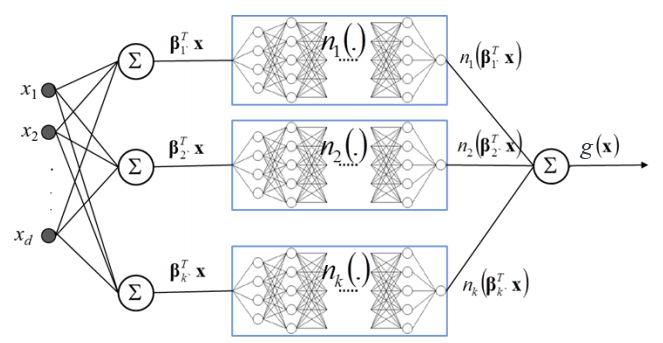
\includegraphics[width=8cm]{img/xnn_arch.png}
	\caption{A diagram of an XNN with three metalayers: the bottom combination layer with  $K$ linear $\sum_j\beta_{k,j}x_j$ hidden units, the middle metalayer with with $K$ hidden and separate $n_k$ ridge functions, and the output combination layer that generates $g^{\text{XNN}}$ predictions. Figure adapted from \citet{wf_xnn}.}
	\label{fig:xnn_arch}
\end{figure}  

\noindent $g^{\text{XNN}}$ is comprised of 3 meta-layers:

\begin{enumerate}[leftmargin=*,labelsep=4.9mm]
	\item The first and deepest meta-layer, composed of $K$ linear $\sum_j\beta_{k,j}x_j$ hidden units, which should learn higher magnitude weights for important $X_j$, is known as the \textit{projection layer}. It is fully connected to each input $X_j$. Each hidden unit in the projection layer may optionally include a bias term.
	\item The second meta-layer contains $K$ hidden and separate $n_k$ ridge functions, or \textit{subnetworks}. Each $n_k$ is a neural network, which can be parameterized to suit a given modeling task. To facilitate direct interpretation and visualization, the input to each subnetwork is the 1-dimensional output of its associated projection layer hidden unit, $\sum_j\beta_{k,j}x_j$. Each $n_k$ can contain several bias terms.
	\item The output meta-layer, called the \textit{combination layer}, is another linear unit comprised of a global bias term, $\mu_0$, and the $K$ weighted 1-dimensional outputs of each subnetwork, $\gamma_kn_k(\sum_j\beta_{k,j}x_j)$. Again, subnetwork output is restricted to 1-dimension for interpretation and visualization purposes.
\end{enumerate}

\subsection{One-dimensional Partial Dependence and Individual Conditional Expectation Details}\label{a_ssec:pd_ice}

Following \citet{esl} a single feature $X_j \in \mathbf{X}$ and its complement set $\mathbf{X}_{\mathcal{P} \setminus \{j\}} \in \mathbf{X}$ (where $X_j \cup \mathbf{X}_{\mathcal{P} \setminus \{j\}} = \mathbf{X}$) is considered. $\text{PD}(X_j, g)$ for a given feature $X_j$ is estimated as the average output of the learned function $g(\mathbf{X})$ when all the observations of $X_j$ are set to a constant $x \in \mathcal{X}$ and $\mathbf{X}_{\mathcal{P} \setminus \{j\}}$ is left unchanged. $\text{ICE}(x_j, g)$ for a given instance $\mathbf{x}$ and feature $x_j$ is estimated as the output of $g(\mathbf{x})$ when $x_j$ is set to a constant $x \in \mathcal{X}$ and all other features $\mathbf{x} \in \mathbf{X}_{\mathcal{P} \setminus \{j\}}$ are left untouched. PD and ICE curves are usually plotted over some set of constants $x \in \mathcal{X}$, as displayed in Subsection \ref{ssec:int_ex_mort} and Appendix \ref{a_ssec:int_ex_sim}. Due to known problems for PD in the presence of strong correlation and interactions, PD should not be used alone. PD should be paired with ICE or be replaced with accumulated local effect (ALE) plots \cite{ice_plots}, \cite{ale_plot}.

\subsection{Shapley Value Details}\label{a_ssec:shap}

For some instance $\mathbf{x} \in \mathcal{X}$, Shapley explanations take the form: 

\begin{equation}
\label{eq:shap_additive}
\begin{aligned}
g(\mathbf{x}) = \phi_0 + \sum_{j=0}^{j=\mathcal{P} - 1} \phi_j \mathbf{z}_j
\end{aligned}
\end{equation}

\noindent In Equation \ref{eq:shap_additive}, $\mathbf{z} \in \{0,1\}^\mathcal{P}$ is a binary representation of $\mathbf{x}$ where 0 indicates missingness. Each $\phi_j$ is the local feature contribution value associated with $x_j$, and $\phi_0$ is the average of $g(\mathbf{X})$. Each $\phi_j$ is a weighted combination of model scores, $g_x(\mathbf{x})$, with $x_j$, $g_x(S \cup \{j\})$, and the model scores without $x_j$, $g_x(S)$, for every subset of features $S$ not including $j$, $S \subseteq \mathcal{P} \setminus \{j\}$, where $g_x$ incorporates the mapping between $\mathbf{x}$ and the binary vector $\mathbf{z}$. 

\begin{equation}
\label{eq:shap_contrib}
\begin{aligned}
\phi_{j} = \sum_{S \subseteq \mathcal{P} \setminus \{j\}}\frac{|S|!(\mathcal{P} -|S| -1)!}{\mathcal{P}!}[g_x(S \cup \{j\}) - g_x(S)]
\end{aligned}
\end{equation}

\noindent Local, per-instance explanations using Shapley values tend to involve ranking $x_j$ by $\phi_j$ values or delineating a set of the $X_j$ names associated with the $k$-largest $\phi_j$ values for some $\mathbf{x}$, where $k$ is some small positive integer, say 5. Global explanations are typically the absolute mean of the $\phi_j$ associated with a given $X_j$ across all of the observations in some set $\mathbf{X}$.

\section{Types of Machine Learning Discrimination in US Legal and Regulatory Settings}\label{a_sec:types}

It is important to explain and draw a distinction between the two major types of discrimination recognized in US legal and regulatory settings, disparate treatment (DT), and disparate impact (DI). DT (which is loosely referred to as \textit{intentional discrimination}) occurs most often in an algorithmic setting when a model explicitly uses protected class status (e.g., race, sex) as an input feature or uses a feature that is so similar to protected class status that it essentially proxies for class membership.  With some limited exceptions, the use of these factors in an algorithm is illegal under several statutes in the US.\textsuperscript{4} DI, colloquially known as \textit{unintentional discrimination}, occurs when some element of a decisioning process includes a \textit{facially neutral} factor (i.e, a reasonable and valid predictor of response) that results in a disproportionate share of a protected class receiving an unfavorable outcome.  In modeling, this is most typically driven by a statistically important feature that is distributed unevenly across classes, which causes more frequent unfavorable outcomes for the protected class.  However, other factors, such as hyperparameter or algorithm choices, can drive DI.  Crucially, legality hinges on whether changing the model, for example exchanging one feature for another or altering the hyperparameters of an algorithm, can lead to a similarly predictive model with lower DI.

\section{Practical vs. Statistical Significance for Discrimination Testing}\label{a_sec:prac_v_stat}

A finding of \textit{practical significance} means that discovered disparity is not only statistically significant, but also passes beyond a chosen threshold that would constitute \textit{prima facia} evidence of illegal discrimination.  Practical significance acknowledges that any large dataset is likely to show statistically significant differences in outcomes by class, even if those differences are not truly meaningful.  It further recognizes that there are likely to be situations where differences in outcomes are beyond a model user’s ability to correct them without significantly degrading the quality of the model. Moreover, practical significance is also needed by model builders and compliance personnel to determine whether a model should undergo remediation efforts before it is put into production. Unfortunately, guidelines for practical significance, i.e., the threshold at which any statistically significant disparity would be considered evidence of illegal discrimination, are not as frequently codified as the standards for statistical significance.  One exception, however, is in employment discrimination analyses, where the US Equal Employment Opportunity Commission (EEOC) has stated that if the AIR is below 0.80 and statistically significant, then this constitutes \textit{prima facia} evidence of discrimination, which the model user must rebut in order for the DI not to be considered illegal discrimination.\footnote{Importantly, the standard of 0.80 is not a law, but a rule of thumb for agencies tasked with enforcement of discrimination laws.  ``Adoption of Questions and Answers To Clarify and Provide a Common Interpretation of the Uniform Guidelines on Employee Selection Procedures,'' Federal Register, Volume 44, Number 43 (1979).} It is important to note that the 0.80 measure of practical significance, also known as the \textit{80\% rule} and the \textit{4/5ths rule}, is explicitly used in relation to AIR, and it is not clear that the use of this threshold is directly relevant to testing fairness for measures other than the AIR.

The legal thresholds for determining statistical significance is clearer and more consistent than that for practical significance.  The first guidance in US courts occurred in a case involving discrimination in jury selection, \textit{Castaneda vs. Partida}.\footnote{\textit{Castaneda vs. Partida}, 430 US 482 - Supreme Court (1977)}   Here, the US Supreme Court wrote that, ``As a general rule for such large samples, if the difference between the expected value and the observed number is greater than two or three standard deviations, then the hypothesis that the jury drawing was random would be suspect to a social scientist.''  This ``two or three standard deviations'' test was then applied to employment discrimination in \textit{Hazelwood School Districts vs. United States.}\footnote{\textit{Hazelwood School Dist. vs. United States}, 433 US 299 (1977)} Out of this, a 5\% two-sided test (z=1.96), or an equivalent 2.5\% one-sided test, has become a common standard for determining whether evidence of disparities is statistically significant.

\section{Additional Simulated Data Results}\label{a_sec:res_sim}

As seen in Subsection \ref{ssec:c_v_uc_sim}, little or no trade-off is required in terms of model to fit to use the constrained models. Hence, intrinsic interpretability, post-hoc explainability, and discrimination are explored further for the $g^\text{MGBM}$ and $g^\text{XNN}$ models in Appendices \ref{a_ssec:int_ex_sim} - \ref{a_ssec:dis_sim}. Intrinsic interpretability for $g^\text{MGBM}$ is evaluated with PD and ICE, and post-hoc explainability is highlighted via global and local Shapley explanations. For $g^\text{XNN}$, Shapley explanation techniques are also used to generate global and local feature importance to augment interpretability results exhibited in Subection \ref{ssec:xnn_sim}. Both $g^\text{MGBM}$ and $g^\text{XNN}$ are evaluated for discrimination using AIR, ME, SMD, and other measures.

\subsection{Interpretability and Post-hoc Explanation Results}\label{a_ssec:int_ex_sim}

Global mean absolute Shapley value feature importance for $g^{\text{MGBM}}(\mathbf{X})$ on the simulated test data is displayed in Figure \ref{fig:sim_mgbm_glob}. 

\begin{figure}[htb]
	\centering
	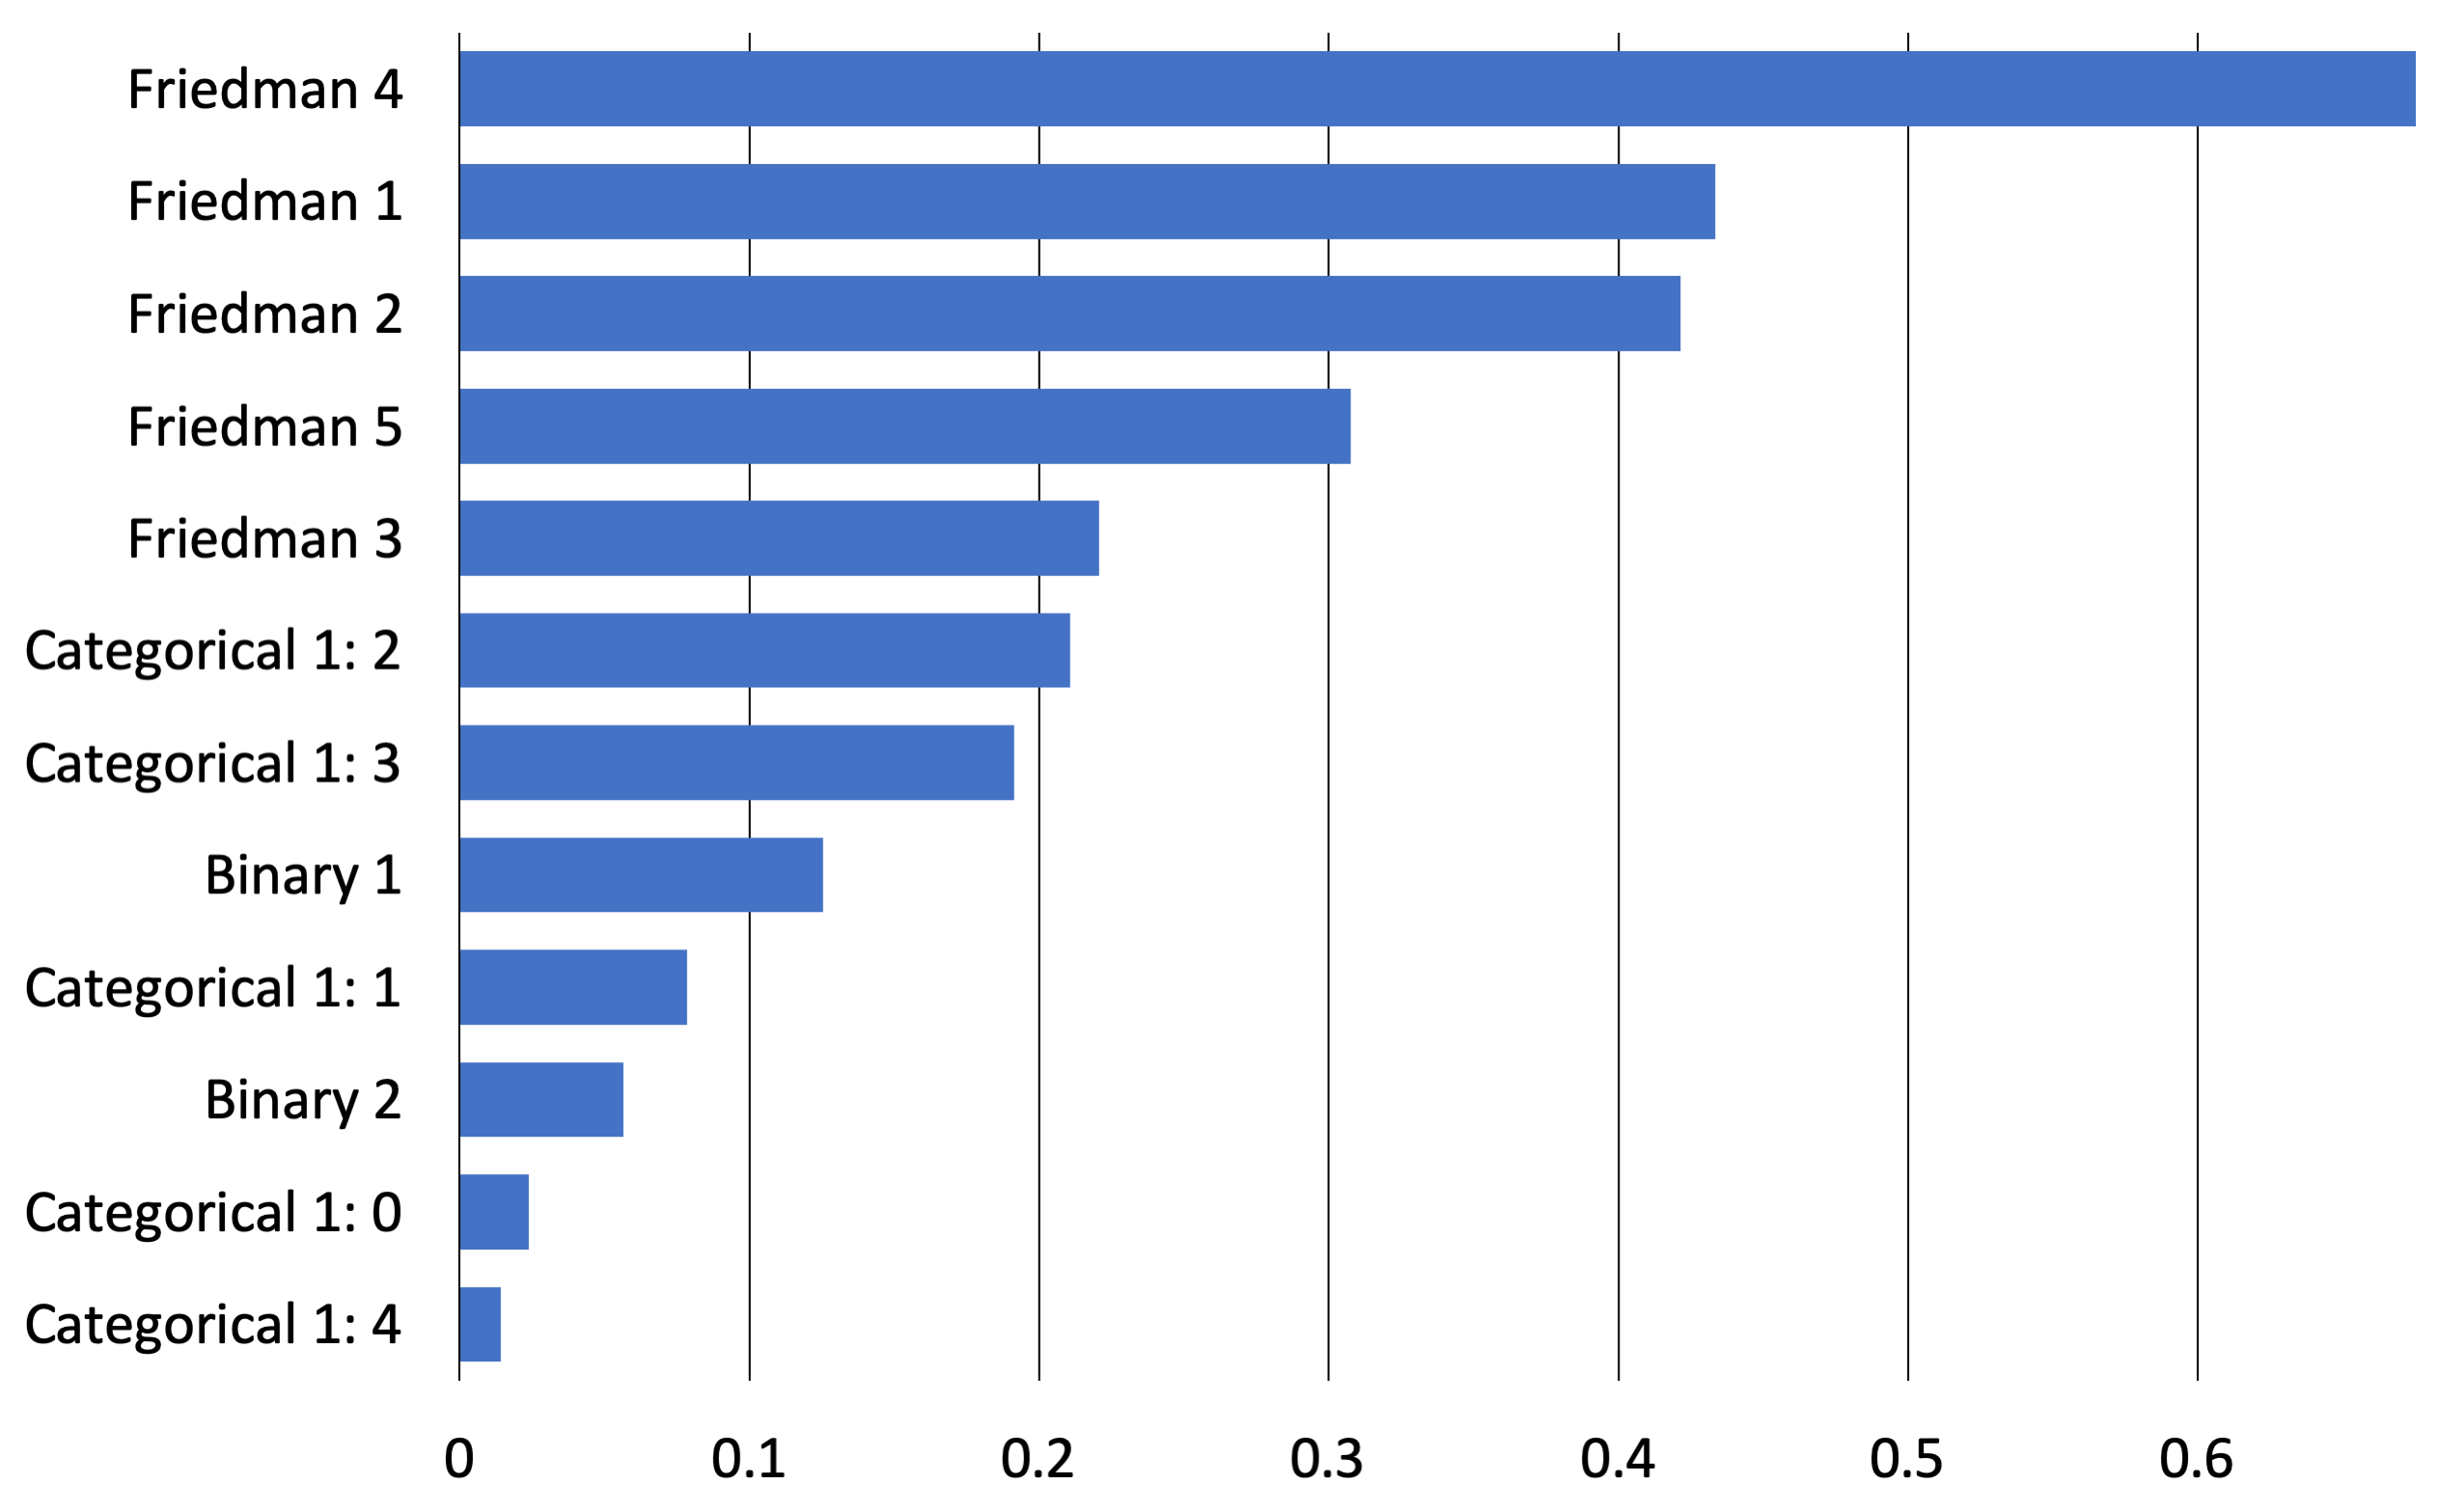
\includegraphics[width=8cm]{img/sim_mgbm_glob.png}
	\caption{Global mean absolute Tree SHAP feature importance for $g^\text{MGBM}(\mathbf{X})$ on the simulated test data.}
	\label{fig:sim_mgbm_glob}
\end{figure}  

\noindent As expected, the $X_{\text{Friedman},j}$ features from the original \citet{friedman1979tree} and \citet{friedman1991multivariate} formula are the main drivers of $g^\text{MGBM}(\mathbf{X})$ predictions, with encoded versions of the augmented categorical and binary features contributing less on average to $g^\text{MGBM}(\mathbf{X})$ predictions. 

Figure \ref{fig:sim_mgbm_glob_pdp_ice} highlights PD, ICE, and histograms of the most important features from Figure \ref{fig:sim_mgbm_glob}. 

\begin{figure}[htb]
	\centering
	\includegraphics[width=15cm]{img/sim_mgbm_glob_pdp_ice.png}
	\caption{PD, ICE for 10 observations across selected percentiles of $g^\text{MGBM}(\mathbf{X})$, and histograms for the three most important input features of $g^\text{MGBM}$ on the simulated test data.}
	\label{fig:sim_mgbm_glob_pdp_ice}
\end{figure}   

$X_{\text{Friedman},1}$, $X_{\text{Friedman},2}$, and $X_{\text{Friedman},4}$ were positively monotonically constrained under $g^\text{MGBM}$ for the simulated data, and positive monotonicity looks to be confirmed on average with PD and at numerous local percentiles of $g^\text{MGBM}(\mathbf{X})$ with ICE. Also, as the PD curves generally follow the patterns of the ICE curves, PD is likely an accurate representation of average feature behavior for $X_{\text{Friedman},1}$, $X_{\text{Friedman},2}$, and $X_{\text{Friedman},4}$. Since PD and ICE curves do not obviously diverge, $g^\text{MGBM}$ is probably not modeling strong interactions, despite the fact that known interactions are included in the simulated data signal generating function in Equation \ref{eq:sim}. The one-dimensional monotonic constraints may hinder the modeling of such interactions, but do not strongly affect overall $g^\text{MGBM}$ accuracy, perhaps due to noise in the simulated data. This is an interesting result for responsible ML practitioners. In some noisy scenarios, monotonicity constraints can increase model interpretability without causing a drastic drop in model accuracy, even when known interactions and non-monotonic behavior exist in training data.

Local Shapley values for records at the 10\textsuperscript{th}, 50\textsuperscript{th}, and 90\textsuperscript{th} percentiles of $g^\text{MGBM}(\mathbf{X})$ in the simulated test data are displayed in Figure \ref{fig:sim_mgbm_loc}. 

\begin{figure}[htb]
	\centering
	\includegraphics[width=15cm]{img/sim_mgbm_loc.png}
	\caption{Tree SHAP values for three observations across selected percentiles of $g^\text{MGBM}(\mathbf{X})$ for the simulated test data.}
	\label{fig:sim_mgbm_loc}
\end{figure}   

\noindent The Shapley values in Figure \ref{fig:sim_mgbm_loc} appear to be a logical result. For the lower prediction at the 10\textsuperscript{th} percentile of $g^\text{MGBM}(\mathbf{X})$, the largest local contributions are negative and the majority of local contributions are also negative. At the median of $g^\text{MGBM}(\mathbf{X})$, local contributions are roughly split between positive and negative values, and at the 90\textsuperscript{th} of $g^\text{MGBM}(\mathbf{X})$, most large contributions are positive. In each case, large local contributions generally follow global importance results in Figure \ref{fig:sim_mgbm_glob} as well.

Figure \ref{fig:sim_xnn_glob} shows global mean absolute Shapley feature importance for $g^\text{XNN}$ on the simulated test data, using the approximate Deep SHAP technique.  

\begin{figure}[htb]
	\centering
	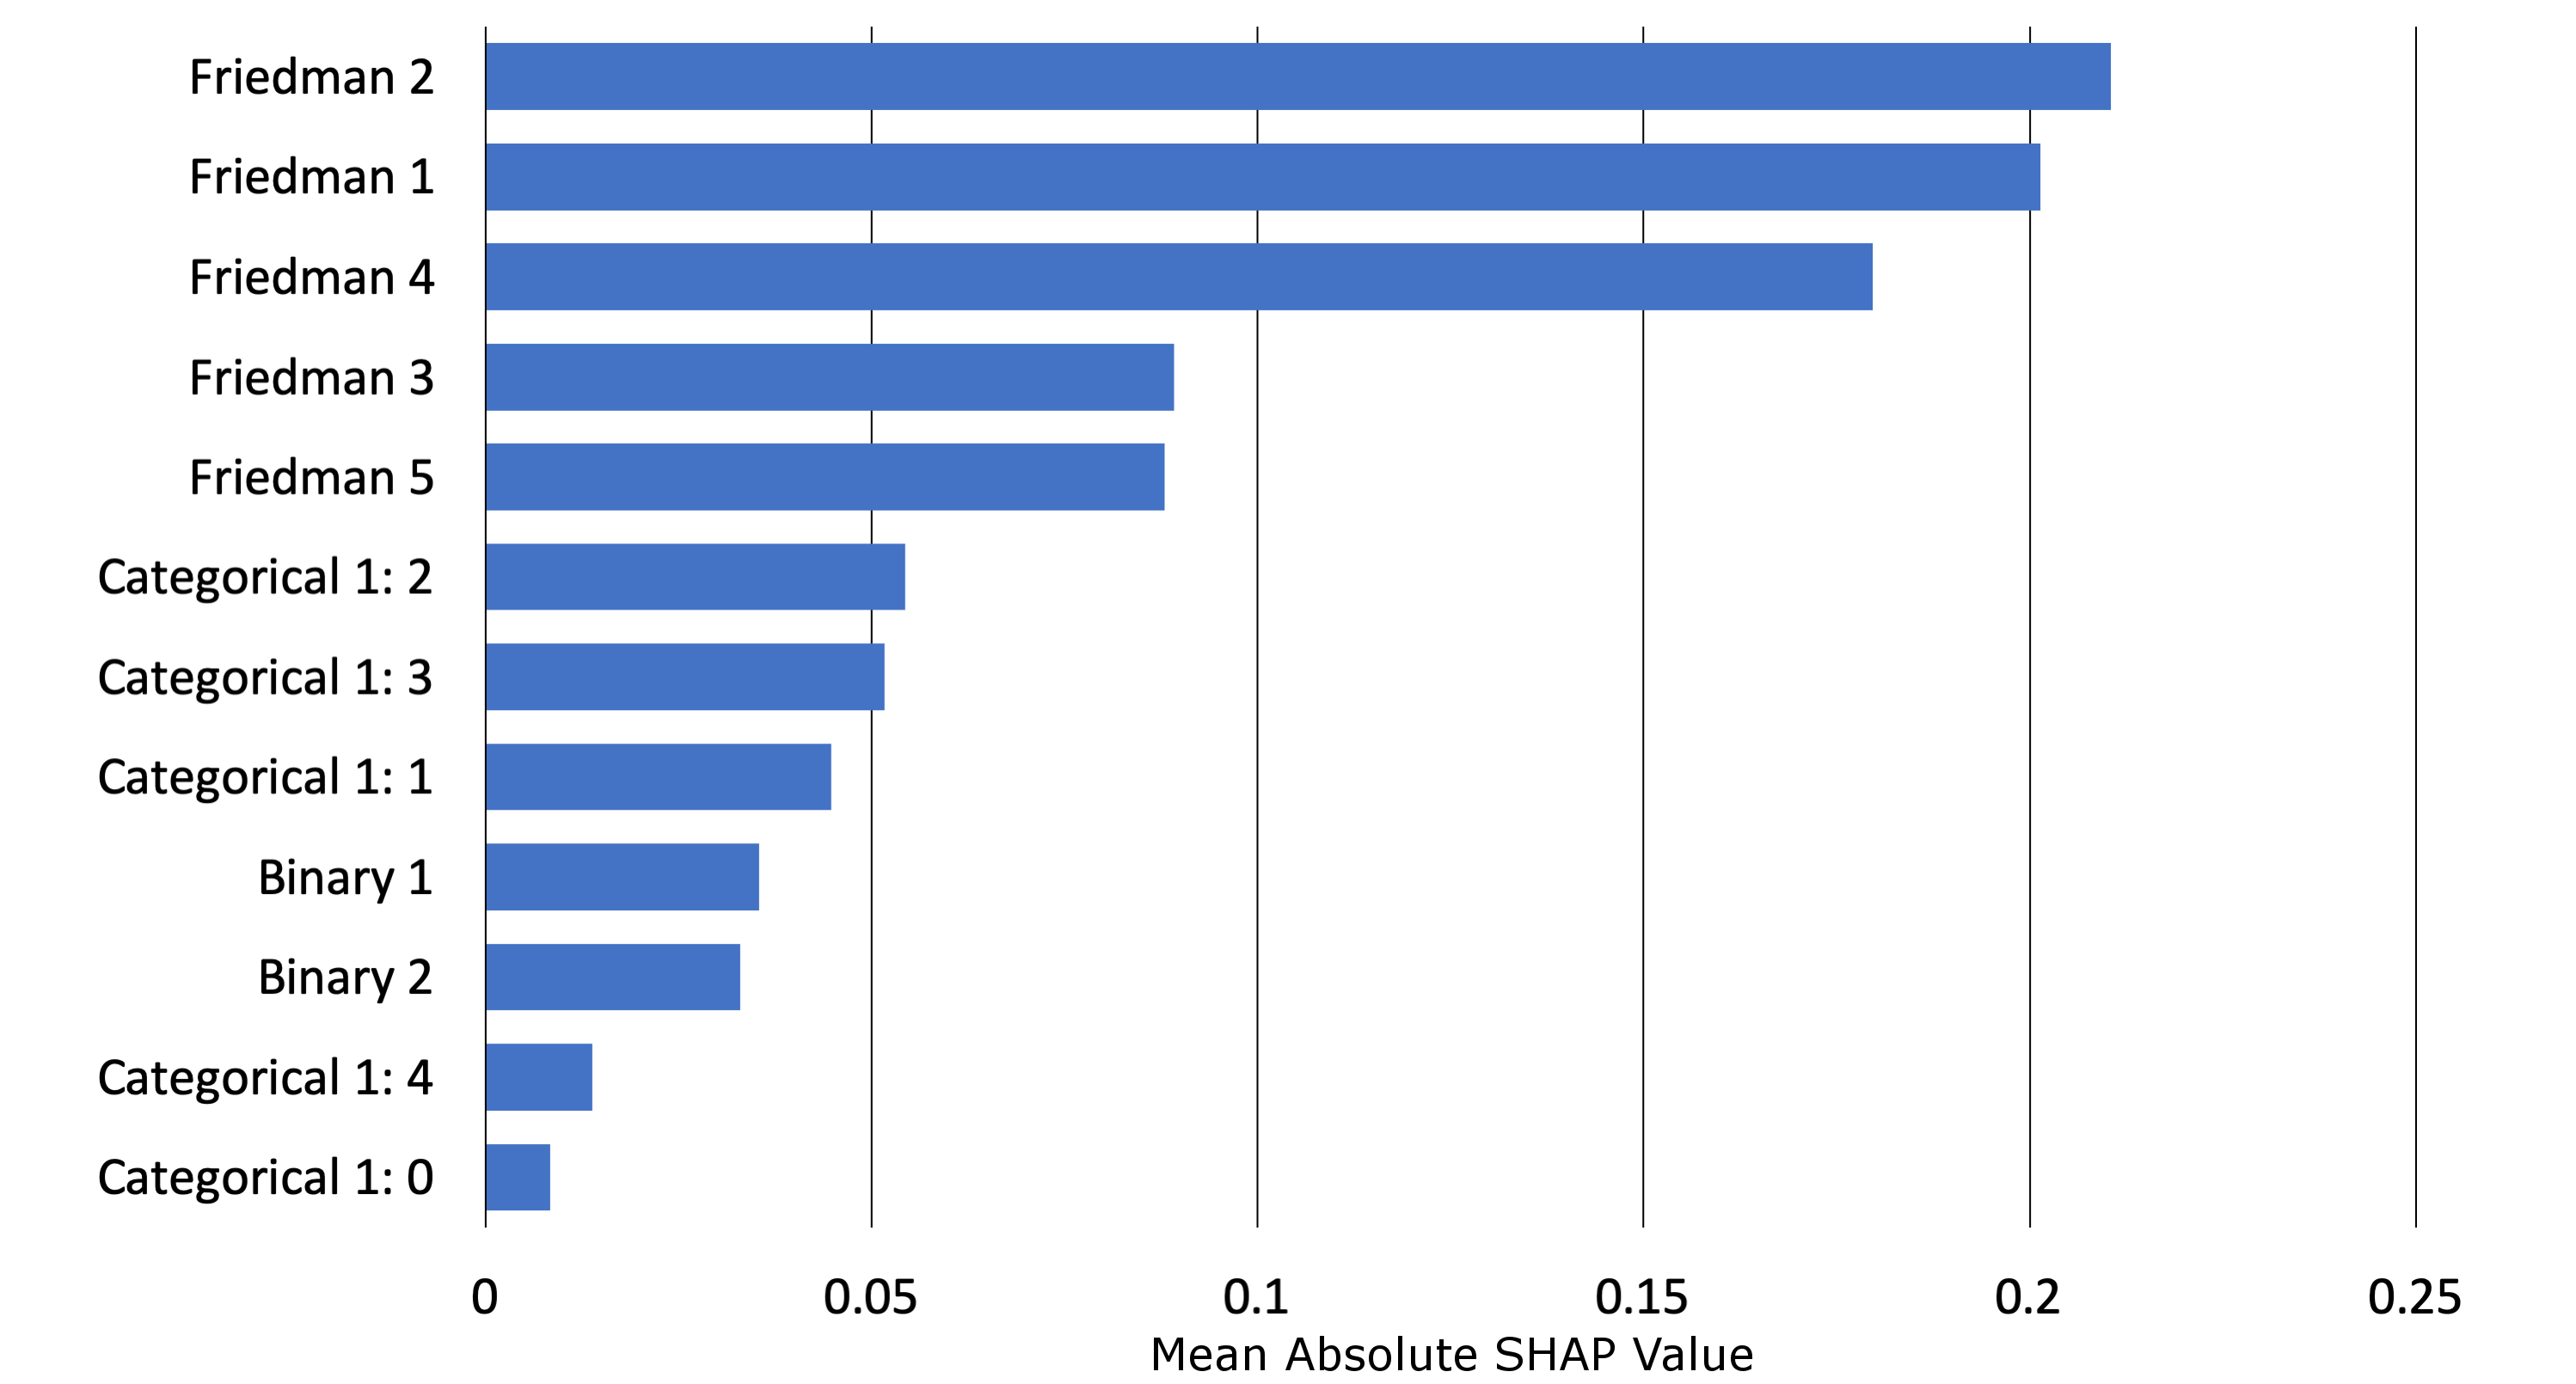
\includegraphics[width=8cm]{img/sim_xnn_glob.png}
	\caption{Global mean Deep SHAP feature importance for $g^\text{XNN}(\mathbf{X})$ on the simulated test data.}
	\label{fig:sim_xnn_glob}
\end{figure} 

\noindent Like $g^\text{MGBM}$, $g^\text{XNN}$ ranks the $X_{\text{Friedman},j}$ features higher in terms of importance than the categorical and binary features. The consistency between the feature rankings of $g^\text{MGBM}$ and $g^\text{XNN}$ is somewhat striking, given their different hypothesis families and architectures. Both $g^\text{MGBM}$ and $g^\text{XNN}$ rank $X_{\text{Friedman},1}$, $X_{\text{Friedman},2}$, and $X_{\text{Friedman},4}$ as the most important features, both place $X_{\text{Categorical},2}$ and $X_{\text{Categorical},3}$ above the $X_{\text{Binary},1}$ and $X_{\text{Binary},2}$ features, both rank $X_{\text{Binary},1}$ above $X_{\text{Binary},2}$, and both place the least importance on $X_{\text{Categorical},4}$ and $X_{\text{Categorical},0}$. 

Local Deep SHAP feature importance in Figure \ref{fig:sim_xnn_loc} supplements the global interpretability of $g^\text{XNN}$ displayed in Figures \ref{fig:sim_xnn_glob} and \ref{fig:sim_xnn_glob_ridge}. Local Deep SHAP values are extracted from the projection layer of $g^\text{XNN}$ and reported in the probability space. Deep SHAP values can be calculated for any arbitrary $g^\text{XNN}(\mathbf{x})$, allowing for detailed, local summarization of individual model predictions. 

\begin{figure}[htb]
	\centering
	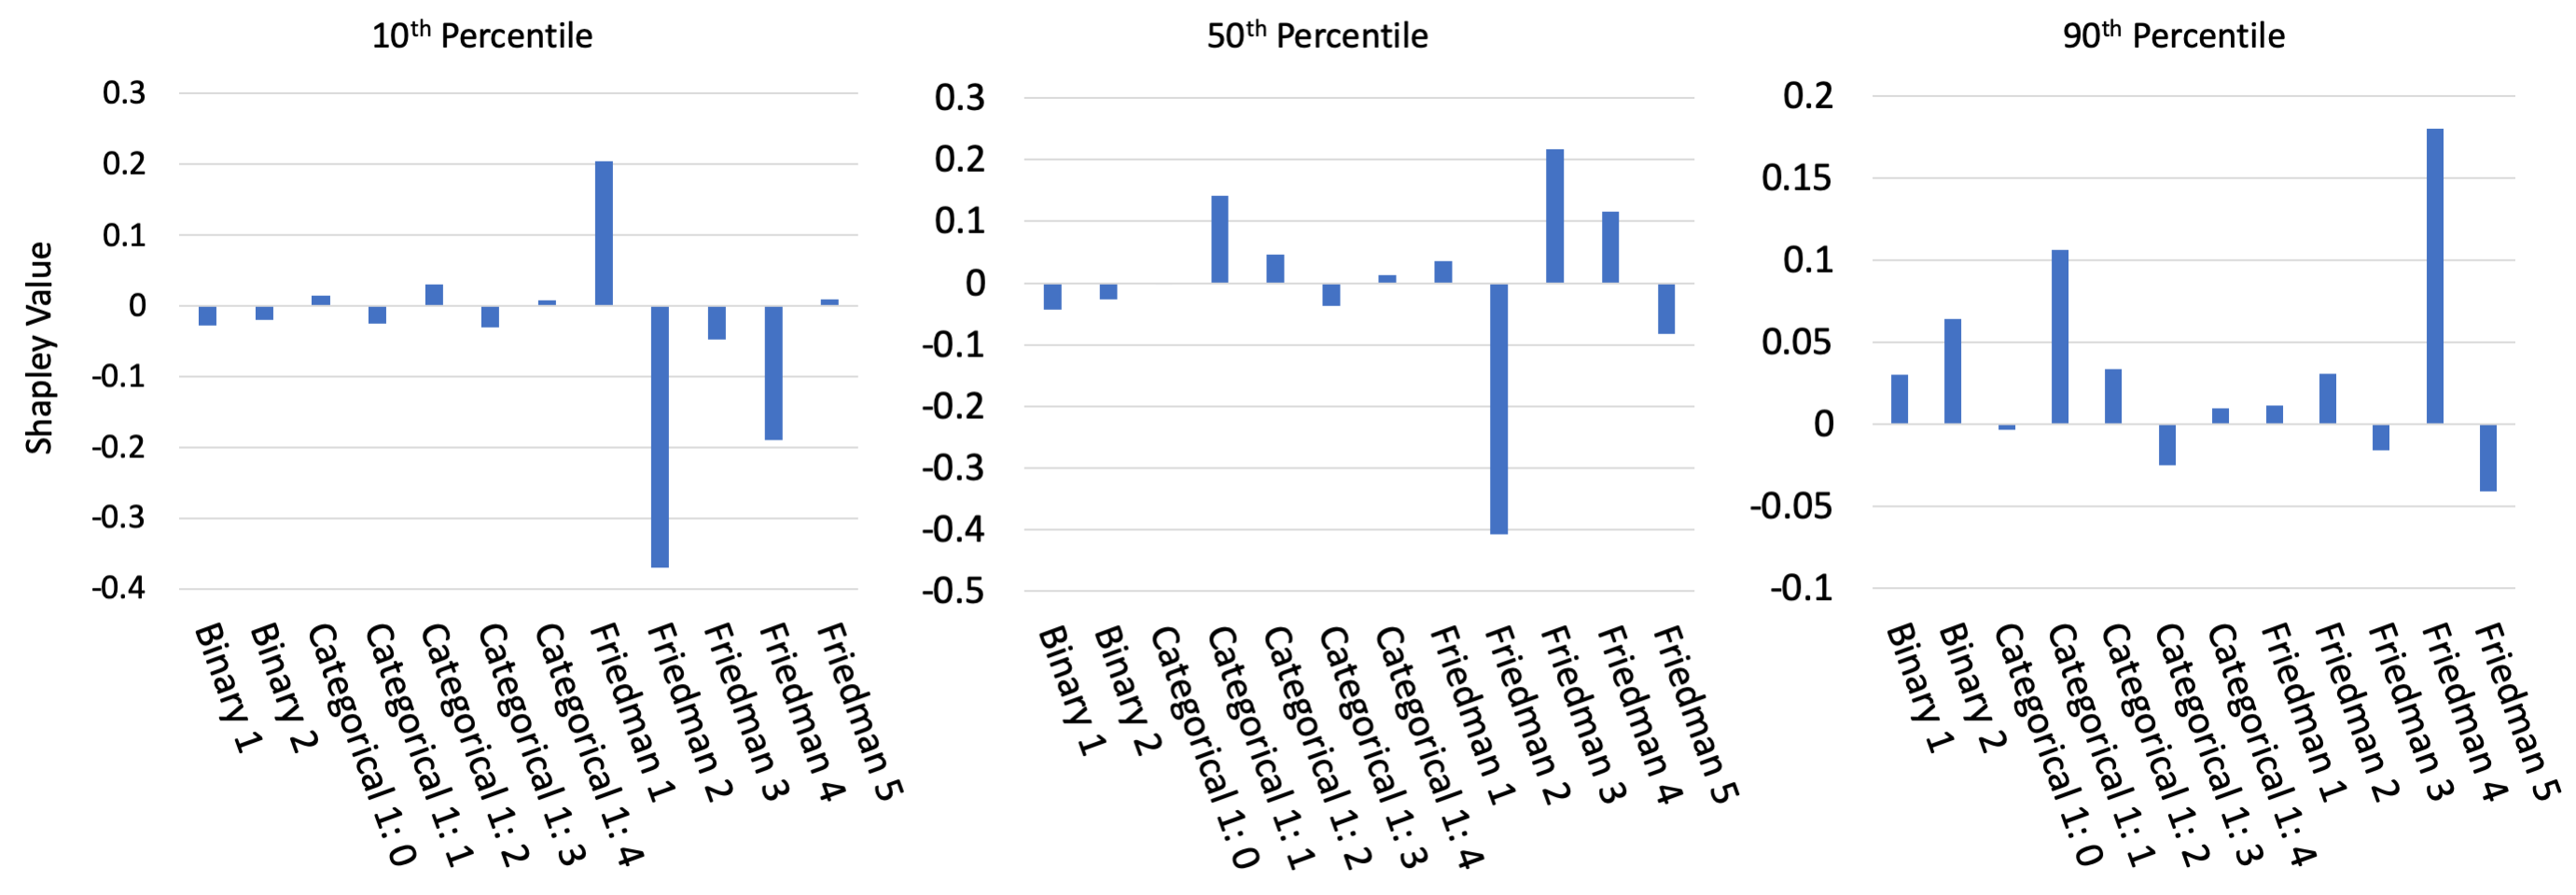
\includegraphics[width=15cm]{img/sim_xnn_loc.png}
	\caption{Deep SHAP values for three observations across selected percentiles of $g^\text{XNN}(\mathbf{X})$ on the simulated test data.}
	\label{fig:sim_xnn_loc}
\end{figure}  

\noindent As expected, Deep SHAP values generally increase from the 10\textsuperscript{th} percentile of $g^\text{XNN}(\mathbf{X})$ to the 90\textsuperscript{th} percentile of $g^\text{XNN}(\mathbf{X})$, with primarily important global drivers of model behavior contributing to the selected local $g^\text{XNN}(\mathbf{x}^{(i)})$ predictions.

\subsection{Discrimination Testing Results}\label{a_ssec:dis_sim}

Tables \ref{tab:sim_disc}\textbf{a} and \ref{tab:sim_disc}\textbf{b} show the results of the disparity tests using the simulated data for two hypothetical sets of class-control groups.  Several measures of disparities are shown, with the SMDs calculated using the probabilities from $g^{\text{MGBM}}$ and  $g^{\text{XNN}}$, false negative rates (FNRs), their ratios, MEs, and AIRs calculated using a binary outcome based on a cutoff of 0.6 (anyone with probabilities of 0.6 or greater receives the favorable outcome).\textsuperscript{11}

Since $g^{\text{MGBM}}$ and $g^{\text{XNN}}$ assume that a higher score is favorable (as might be the case if the model were predicting responses to marketing offers), one might consider the relative FNRs as a measure of the class-control disparities. Table \ref{tab:sim_disc} shows that protected group 1 has higher relative FNRs under $g^{\text{XNN}}$ (1.13 vs. 1.06).  However, in Table \ref{tab:sim_n_acc} the overall FNRs were lower for  $g^{\text{XNN}}$ (0.357 vs. 0.401). This illustrates a danger in considering relative class-control metrics in isolation when comparing across models: despite the $g^\text{MGBM}$ appearing to be a relatively fairer model, more protected group 1 members experience negative outcomes using $g^{\text{MGBM}}$. This is because FNR accuracy improves for both the protected group 1 and control group 1, but members of control group 1 benefit more than those in protected group 1.  Of course, the choice of which model is truly fairer is a policy question.

\begin{table}[htb]
	\hskip-10pt
	\begin{subtable}{0.45\textwidth}
		\captionsetup{width=7cm}
		\caption{Group size, accuracy, and FNR for $g^\text{MGBM}$ and $g^\text{XNN}$ on the simulated test data.} 
		\centering
		\resizebox{\columnwidth}{!}{%
			\begin{tabular}{ccccc}
				\toprule
		\textbf{Class} & $\mathbf{N}$ & \textbf{Model} & \textbf{Accuracy}$\uparrow$ & \textbf{FNR}$\downarrow$ \\
				\midrule
				Protected 1	& 3,057 & \begin{tabular}{@{}c@{}} $g^\text{MGBM}$ \\ $g^\text{XNN}$\end{tabular} & \begin{tabular}{@{}c@{}} 0.770 \\ 0.771\end{tabular} & \begin{tabular}{@{}c@{}} 0.401 \\ 0.357\end{tabular} \\	
				\midrule			 
				Control 1 & 16,943 & \begin{tabular}{@{}c@{}} $g^\text{MGBM}$ \\ $g^\text{XNN}$\end{tabular} & \begin{tabular}{@{}c@{}} 0.739 \\ 0.756\end{tabular} & \begin{tabular}{@{}c@{}} 0.378 \\ 0.314\end{tabular} \\
				\midrule
				Protected 2	& 9,916 & \begin{tabular}{@{}c@{}} $g^\text{MGBM}$ \\ $g^\text{XNN}$\end{tabular} & \begin{tabular}{@{}c@{}} 0.758 \\ 0.762\end{tabular} & \begin{tabular}{@{}c@{}} 0.331 \\ 0.302\end{tabular} \\	
				\midrule
				Control 2 & 10,084 & \begin{tabular}{@{}c@{}} $g^\text{MGBM}$ \\ $g^\text{XNN}$\end{tabular} & \begin{tabular}{@{}c@{}} 0.729 \\ 0.756\end{tabular} & \begin{tabular}{@{}c@{}} 0.420 \\ 0.332\end{tabular} \\		
				\bottomrule
				\label{tab:sim_n_acc}
			\end{tabular}%
		}
	\end{subtable}
	\hspace{5pt}
	\begin{subtable}{0.45\textwidth}
		\vspace{-11pt}
		\captionsetup{width=10cm}
		\caption{%
			\leftskip=45pt
			AIR, ME, SMD, and FNR ratio for $g^\text{MGBM}$ and $g^\text{XNN}$ on the simulated test data.}
		\centering
		\scalebox{0.95}{
			\begin{tabular}{ccccccc}
				\toprule
		\textbf{Model} &  \begin{tabular}[x]{@{}c@{}}\textbf{Protected}\\\textbf{Class}\end{tabular} & \begin{tabular}[x]{@{}c@{}}\textbf{Control}\\\textbf{Class}\end{tabular} & \textbf{AIR}$\uparrow$ & \textbf{ME}$\downarrow$ & \textbf{SMD}$\downarrow$ & \begin{tabular}[x]{@{}c@{}}\textbf{FNR}\\\textbf{Ratio}\end{tabular}$\downarrow$\\
				\midrule
				$g^\text{MGBM}$	& \begin{tabular}{@{}c@{}} 1 \\  2\end{tabular}	& \begin{tabular}{@{}c@{}} 1 \\ 2\end{tabular}	& \begin{tabular}{@{}c@{}} 0.752 \\ 1.10\end{tabular} & \begin{tabular}{@{}c@{}} 9.7\% \\ -3.6\%\end{tabular}	& \begin{tabular}{@{}c@{}} -0.206 \\ 0.106\end{tabular}	& \begin{tabular}{@{}c@{}} 1.06 \\ 0.788\end{tabular}\\
				\midrule 
				$g^\text{XNN}$ & \begin{tabular}{@{}c@{}} 1 \\ 2\end{tabular} & \begin{tabular}{@{}c@{}} 1 \\  2\end{tabular}	& \begin{tabular}{@{}c@{}} 0.727 \\ 0.976\end{tabular}	& \begin{tabular}{@{}c@{}} 12.0\%\\ 1.0\%\end{tabular}	& \begin{tabular}{@{}c@{}} -0.274 \\ 0.001\end{tabular}	& \begin{tabular}{@{}c@{}} 1.13 \\ 0.907\end{tabular} \\										
				\bottomrule
				\label{tab:sim_disc_detail}
			\end{tabular}
		}
	\end{subtable}
	\captionsetup{width=10cm}
	\caption{Discrimination measures for the simulated test data. Arrows indicate the direction of improvement for each measure.}
	\label{tab:sim_disc}
\end{table}

For $g^{\text{XNN}}$, 12.0\% fewer control group 1 members receive the favorable offer under the ME column in Table \ref{tab:sim_disc}. Of note is that 12.0\% is not a meaningful difference without context.  If the population of control group 1 and control group 2 were substantially similar in relevant characteristics, 12.0\% could represent an extremely large difference and would require remediation.  But if they represent substantially different populations, then 12.0\% could represent a reasonable deviation from parity.  As an example, if a lending institution that has traditionally focused on high credit quality clients were to expand into previously under-banked communities, an 12.0\% class-control difference in loan approval rates might be expected because the average credit quality of the new population would be lower than that of the existing population. Protected group 1’s AIR under $g^\text{XNN}$ is 0.727, below the EEOC 4/5ths rule threshold.  It is also highly statistically significant (not shown, but available in resources discussed in Subsection \ref{ssec:soft}). Together these would indicate that there may be evidence of illegal DI.  As with ME and other measures, the reasonableness of this disparity is not clear outside of context.  However, most regulated institutions that do perform discrimination analyses would find an AIR of this magnitude concerning and warranting further review. Some pertinent remediation strategies for discovered discrimination are discussed in Subsection \ref{ssec:disc_rem}.

SMD is used here to measure $g^\text{MGBM}(\mathbf{X})$ and $g^\text{MGBM}(\mathbf{X})$ probabilities prior to being transformed into classifications.  (This measurement would be particularly relevant if the probabilities are used in combination with other models to determine an outcome.)  The results show that $g^\text{MGBM}$ has less DI than $g^\text{XNN}$ (-0.206 vs. -0.274), but both are close to Cohen’s small effect threshold of -0.20. Whether a small effect would be a highlighted concern would depend on a organization’s chosen threshold for flagging models for further review. 

\section{Discrimination Testing and Cutoff Selection}\label{a_sec:cut}

The selection of which cutoff to use in production is typically based on the model’s use case, rather than one based solely on the statistical properties of the predictions themselves.  For example, a model developer at a bank might build a credit model where the F1 score is maximized at a delinquency probability cutoff of 0.15.  For purposes of evaluating the quality of the model, she may review confusion matrix statistics (accuracy, recall, precision, etc.) using cutoffs based on the maximum F1 score. But, because of its risk tolerance and other factors, the bank itself might be willing to lend to anyone with a delinquency probability of 0.18 or lower, which would mean that anyone who is scored at 0.18 or lower would receive an offer of credit.  Because disparity analyses are concerned with how people are affected by the deployed model, it is essential that any confusion matrix-based metrics of disparity be calculated on the in-production classification decisions, rather than the cutoffs that are not related to what those affected by the model will experience.

\section{Recent Fairness Techniques in US Legal and Regulatory Settings}\label{a_sec:comp}

Great care must be taken in order to ensure that the appropriate fairness metrics are chosen, because certain metrics may not be appropriate for some use cases. Additionally, the effects of changing the model must be viewed holistically.  For example, the mortgage data disparity analysis in Subsection \ref{ssec:dis_mort} shows that if one were to choose $g^\text{MGBM}$ over $g^\text{XNN}$ because $g^\text{MGBM}$ has a lower FPR ratio for blacks, it would ultimately lead to a higher FPR for blacks overall, which may represent doing more harm than good.

Furthermore, using some recently developed discrimination mitigation methods may lead to non-compliance with anti-discrimination laws and regulations.  A fundamental maxim of US anti-discrimination law is that (to slightly paraphrase), ``similarly situated people should be treated similarly.''\footnote{In the pay discrimination case, \textit{Bazemore vs. Friday}, 478 US 385 (1986), the US Supreme Court found that,``Each week's paycheck that delivers less to a black than to a similarly situated white is a wrong actionable ...''  Beyond the obvious conceptual meaning, what specifically constitutes \textit{similarly situated} is controversial and its interpretation differs by circuit.} A model developed without inclusion of class status (or proxies thereof) considers similarly situated people the same on the dimensions included in the model: people who have the same feature values will have the same model output (though there may be some small or random differences in outcomes due to computational issues). Obviously, the inclusion of protected class status will change model output by class. With possible rare exceptions, this is likely to be viewed with legal and regulatory skepticism today, even if including class status is done with fairness as the goal.\footnote{In a reverse discrimination case, \textit{Ricci v Desafano}, 557 US 557 (2009), the court found that any consideration of race which is not justified by correcting for past proven discrimination is illegal and, moreover, a lack of fairness is not necessarily evidence of illegal discrimination.}  Preprocessing and post-processing techniques may be similarly problematic, because industries that must provide explanations to those who receive unfavorable treatment (e.g., adverse action notices in US financial services) may have to incorporate the class adjustments into their explanations as well.

%%%%%%%%%%%%%%%%%%%%%%%%%%%%%%%%%%%%%%%%%%
\reftitle{References}

%=====================================
% References, variant A: external bibliography
%=====================================
\externalbibliography{yes}
\bibliography{article-information-2019}

%%%%%%%%%%%%%%%%%%%%%%%%%%%%%%%%%%%%%%%%%%
\end{document}

